\documentclass{article}


% Options: none = anonymous submission, [preprint] = named arXiv-style,
% [accepted] = camera-ready (also set \openreview below).
\usepackage[preprint]{tmlr}


\usepackage[utf8]{inputenc}
\usepackage[T1]{fontenc}
\usepackage{hyperref}
\usepackage{url}
\usepackage{booktabs}
\usepackage{amsfonts}
\usepackage{amsmath,amssymb}
\usepackage{nicefrac}
\usepackage{microtype}
\usepackage{xcolor}
\usepackage{graphicx}
\usepackage{multirow}
\usepackage{caption}
\usepackage{subcaption}
\usepackage{enumitem}
\usepackage{float}
\usepackage{color}


\graphicspath{{figures/}{../src/analysis/figures/}}


\setlist{nosep,leftmargin=*}


\definecolor{wingreen}{HTML}{1b7a28}
\definecolor{lossred}{HTML}{a6201a}
\newcommand{\win}[1]{\textcolor{wingreen}{\textbf{#1}}}
\newcommand{\loss}[1]{\textcolor{lossred}{#1}}
\newcommand{\tie}[1]{\textbf{#1}}


% Camera-ready only: \def\openreview{\url{https://openreview.net/forum?id=XXXXXXXXXX}}


\title{Teacher-Supervised Failure Detection for Distilled\\Semantic Segmentation under Domain Shift}


\author{\name Shay Manor \email manors@purdue.edu \\
      \addr Department of Computer Science \\
      Purdue University
      \AND
      \name Aniket Bera \email aniketbera@purdue.edu \\
      \addr Department of Computer Science \\
      Purdue University}


\begin{document}
\maketitle
\raggedbottom


\begin{abstract}
Semantic segmentation enables perception in safety-critical systems, but under distribution shift, distilled students frequently emit \emph{silent failures}: predictions that are highly confident yet inaccurate. We operationalise a silent failure at the image level as an image whose segmentation quality (mean IoU) falls in the worst quintile while its mean confidence stays high, and study how well such images can be ranked from a frozen student alone. Existing post-hoc confidence scores (MSP, entropy, MC-Dropout, MaxLogit, energy) read only the student's output distribution and degrade precisely in this high-confidence regime. We introduce a lightweight dense guardrail head---$0.2$--$0.4$M parameters, $2$--$6\%$ of the student---that reads the frozen student's logits and decoder features and, trained with corruption augmentation, flags these failures in a single forward pass without invoking the teacher. This learned head, rather than any single supervision signal, is the main driver of its advantage over post-hoc scores, and it is most reliable at strict confidence thresholds where those scores are weakest: on BDD100K at MSP$\geq$0.97 it improves CF-AUROC by $+22$\,pp over MSP. On top of the head, a controlled comparison isolates the supervision signal: teacher-derived dense targets give a smaller but consistent gain over matched ground-truth targets under shift ($+1.0$ to $+3.5$\,pp at MSP$\geq$0.85, consistent across three matched training seeds, widening to $+5$ to $+11$\,pp at stricter thresholds on ACDC and BDD100K). Finally, passing per-pixel energy and max-logit into the head as input channels fuses learned failure structure with confidence magnitude in one score and beats the energy score by $+2.2$\,pp CF-AUROC on ACDC. Across four datasets, a lightweight learned guardrail---enhanced by teacher supervision and confidence-feature fusion---is an effective single-pass detector of silent failures in distilled segmentation models under distribution shift, at sub-teacher latency.
\end{abstract}


\section{Introduction}

Semantic segmentation enables perception in safety-critical systems such as autonomous driving and robotic manipulation, where each pixel prediction propagates into downstream planning and control. Deploying these models on edge hardware typically relies on knowledge distillation (KD)~\cite{hinton2015distilling}, with structured variants for dense prediction~\cite{liu2019structuredkd}. However, distilled students inherit the teacher's proficiency unevenly. Under domain shift (weather, lighting, camera artifacts), they produce silent confident failures, confident predictions that are wrong, which downstream systems act on without warning. Selective prediction addresses this by abstaining or deferring on unreliable inputs, exchanging coverage for lower prediction risk~\cite{geifman2017selective}. Strong reliability estimates are required for effectiveness. Post-hoc confidence scores (MSP, entropy, MC-Dropout) use the student's output distribution, which is uninformative when the student is confident. MaxLogit correlates with OOD detection but uses logit magnitudes rather than learned failures, and degrades at stricter confidence thresholds where silent failures are most important.

We address this by training a lightweight dense guardrail head ($0.2$--$0.4$M parameters, $2$--$6\%$ of the student) on the frozen student's logits and decoder features to predict per-pixel failures, using corruption augmentation to broaden it beyond clean source-domain inputs. At inference the head produces a single failure score in one forward pass, at sub-teacher latency and without invoking the teacher; this learned head and its training pipeline, rather than any single supervision signal, are the primary source of its advantage over post-hoc confidence scores. Given the head, we then ask a separate, controlled question: does supervising it with teacher-derived dense targets---defined relative to the student's own distilled function rather than to fixed source-domain labels---transfer better under shift than supervising it with ground-truth labels? We train on Cityscapes and evaluate on three out-of-distribution (OOD) benchmarks (ACDC, IDD, BDD100K).


\paragraph{Problem statement.}
We take the deployed system as given: a student $S$ distilled from a teacher $T$ and frozen, running on edge hardware, on inputs drawn from a test distribution that differs from the source domain in ways not known at training time. The task is not to make $S$ more accurate but to say, per image and before any downstream module consumes the prediction, how much that prediction can be trusted. Concretely, we require a scalar score $g(x)$ that ranks images by their true segmentation risk $\rho(x) = 1 - \mathrm{mIoU}(x)$, and we ask how well it ranks the images that the student itself already believes: the subset on which its mean maximum softmax probability is above a confidence threshold $\tau$. That restriction is what makes the problem hard and what makes it matter. On the low-confidence images the student's own probabilities already carry the signal; the failures that survive a high $\tau$ are exactly the ones a confidence threshold cannot remove, and are the ones that reach the planner unflagged.

Three constraints define the setting. The detector must run in a single forward pass at edge latency, so test-time ensembling and multi-pass stochastic estimates are out of budget. It must not invoke the teacher, since a teacher call at test time would defeat the purpose of distillation---the teacher is available during training only, as a source of supervision, and at deployment only as the target of an occasional deferral. And it may not use labels from the shifted domain, since none exist. Everything the detector sees at test time is therefore a function of the frozen student's own forward pass. The question we study is what to \emph{train} that function against.


\paragraph{Contributions.}
\begin{enumerate}
\item A lightweight dense failure detector: a $0.2$--$0.4$M-parameter head on the frozen student's logits and decoder features, trained with corruption augmentation, that flags silent confident failures under domain shift in a single forward pass without the teacher. It is competitive with post-hoc confidence scores and most reliable at strict confidence thresholds, where silent failures are most dangerous and probability-based post-hoc scores (MSP, MC-Dropout) revert toward chance.
\item A controlled comparison of teacher- vs.\ ground-truth-derived supervision: with the head, optimizer, and augmentation held fixed, teacher-derived dense targets give a smaller but consistent improvement over matched ground-truth supervision under shift, largest at strict thresholds ($+1.0$ to $+3.5$\,pp at MSP$\geq$0.85 over three matched seeds, widening to $+5$ to $+11$\,pp on ACDC and BDD).
\item A confidence-feature variant that ingests per-pixel energy and max-logit as input channels, fusing learned failure structure with confidence magnitude into a single score; on ACDC it beats the energy score by $+2.2$\,pp CF-AUROC (paired sign-test $p{=}0.001$), a gain that is separate from, and stacks on, the teacher-vs-GT effect.
\item A cost-reliability analysis: at sub-teacher latency, the single-pass guardrail Pareto-dominates four-pass MC-Dropout on failure detection under shift, while a three-member Deep Ensemble---at several times the training and storage cost---does not improve on it (\S\ref{sec:latency}).
\end{enumerate}


\section{Related Work}

\paragraph{Selective prediction.} Selective prediction abstains on low-confidence inputs, exchanging decreased coverage for lower risk~\cite{geifman2017selective}. Standard post-hoc scores include MSP~\cite{hendrycks2017baseline}, temperature scaling~\cite{guo2017calibration}, MC-Dropout~\cite{gal2016dropout} and MaxLogit~\cite{hendrycks2022scaling}. Classical alternatives are Deep Ensembles~\cite{lakshminarayanan2017deepensembles}, where predictive uncertainty degrades gracefully under distribution shift ~\cite{ovadia2019trust}, and aleatoric/epistemic uncertainty for dense vision~\cite{kendall2017uncertainties}. Learned confidence heads move beyond these post-hoc scores. SelectiveNet jointly trains a predictor and a reject option~\cite{geifman2019selectivenet}, and ConfidNet trains an auxiliary head to predict the True Class Probability from ground-truth labels~\cite{corbiere2019confidnet}. Recent work standardizes measurements for failure detection and warns that it is easily mis-evaluated~\cite{jaeger2023call, traub2024overcoming}; in particular, \citet{traub2024overcoming} show that common multi-threshold summaries including AURC can misrank systems and propose the AUGRC. We report the standard AURC (defined in Appendix~\ref{app:impl}) and confident-failure AUROC, and treat AUGRC as a complementary metric rather than one our AURC subsumes. We evaluate failure \emph{ranking}---ordering images by risk---which is distinct from calibration, the accuracy of predicted failure probabilities; our score is a ranking read-out and we make no calibration claim. Our contribution is empirical rather than architectural: under a fixed lightweight dense head, teacher-relative dense targets outperform source-label targets in the shifted, high-confidence regime, because they are defined relative to the student's distilled function rather than to fixed source-domain labels.

\paragraph{Out-of-distribution and anomaly segmentation.} For dense prediction, reliability is often cast as per-pixel OOD/anomaly detection. Representative approaches include standardized max-logit for road obstacles~\cite{jung2021standardized}, entropy maximization with meta-classification~\cite{chan2021entropy}, resynthesis/reconstruction discrepancy~\cite{dibiase2021pixel}, and predicting a segmentation network's own errors from local adversarial perturbations~\cite{besnier2021triggering}. Deterministic single-pass uncertainty~\cite{mukhoti2023deep}, evidential mask transformers~\cite{schmidt2025prior2former}, and generalize-or-detect training under multiple shifts~\cite{gao2024generalize} pursue the same goal. These methods use a single standalone model, whereas we instead ask whether a teacher used to distill a compressed student also provides a better supervision signal for the student's image-level failure detection under shift. Reducing a dense score to an image-level one is itself consequential: \citet{guarino2026aggregation} show that global mean pooling discards spatial structure and that spatially-aware aggregation improves downstream detection. We hold aggregation fixed (mean pooling) across all methods to isolate the supervision signal.

\paragraph{Uncertainty distillation.} Deep Ensembles transfer uncertainty from ensemble teachers, typically requiring 3--5 independently trained models ~\cite{lakshminarayanan2017deepensembles}. DUDES distills ensemble uncertainty into a single-pass segmentation model ~\cite{landgraf2024dudes}. Our method is complementary and uses only a single teacher and a lightweight head ($0.2$--$0.4$M parameters), rather than distilling ensemble uncertainty.

\paragraph{Knowledge distillation for segmentation.} SegFormer and related architectures are compressed via standard KD ~\cite{hinton2015distilling, xie2021segformer}. Structured KD extends this with pixel-wise, pairwise, and holistic dense-prediction objectives ~\cite{liu2019structuredkd}. Prior work focuses on closing the mIoU gap. Our work complements this by equipping the distilled student with a post-distillation reliability measure.


\section{The Guardrail}

\paragraph{Overview.}
We propose a light guardrail operating on frozen student logits, predicting dense per-pixel student--teacher disagreement and severity. A strong teacher model $T$ (SegFormer-B5) is first used to distill the student $S$. Both networks are then frozen, and we train the guardrail $G$ on top of the student's logits to predict the severity and the student--teacher disagreement. We isolate the effect of the supervision signal by comparing two cases of supervision: (a) teacher-derived dense targets, and (b) ground-truth-derived dense targets, while fixing the guardrail architecture, optimizer, and corruption augmentation.

\begin{figure}[H]
\centering
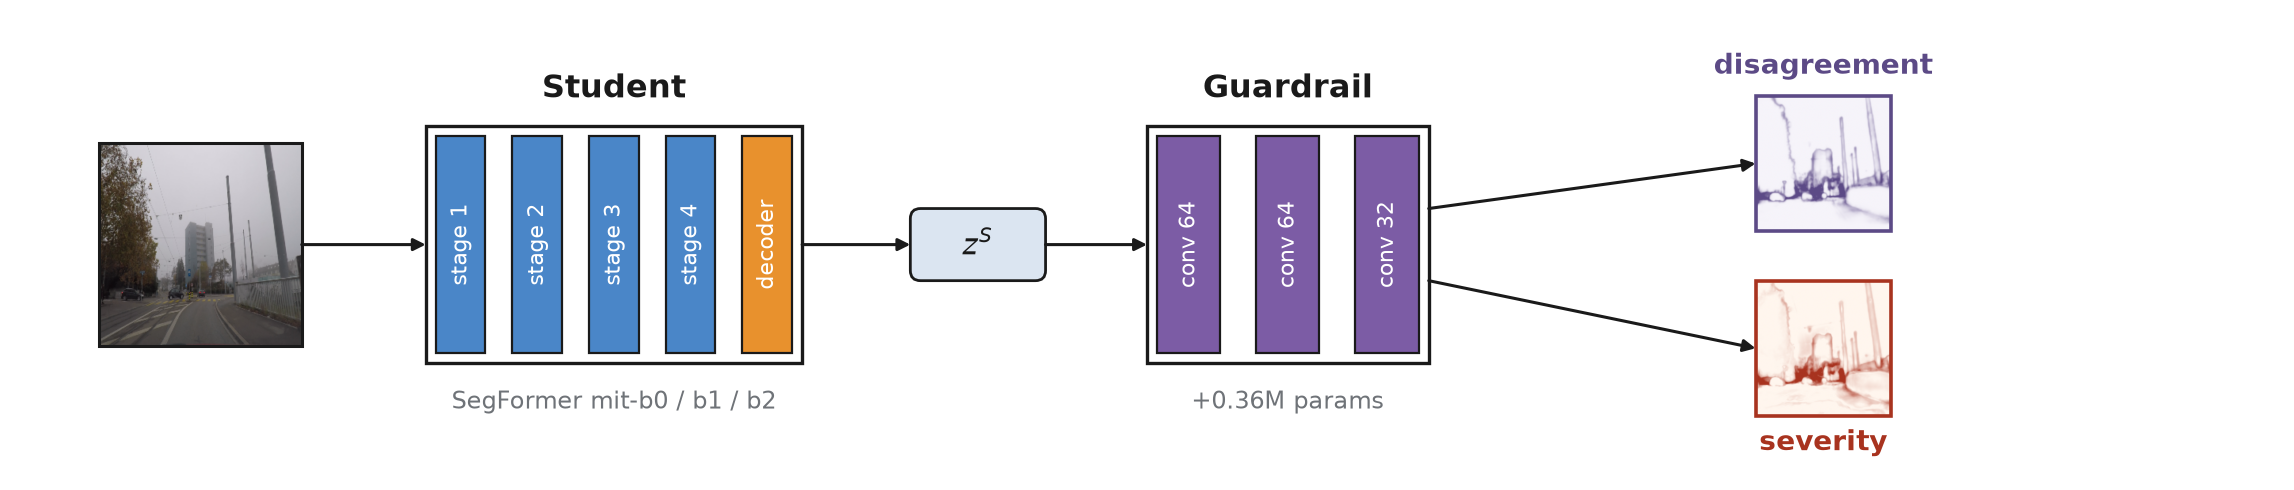
\includegraphics[width=\linewidth]{fig_arch_overview.png}
\caption{Overview of the guardrail pipeline. The guardrail reads the student per-pixel logits ($C{=}19$ channels) concatenated with the student's decoder feature map ($F$; channels${=}256$ for mit-b0, $512$ for b1/b2), and outputs a dense per-pixel map of severity and student--teacher disagreement.}
\label{fig:arch}
\end{figure}


\paragraph{Notation.}
For an input image $x$, let $z^S(x), z^T(x) \in \mathbb{R}^{H \times W \times C}$ denote the student and teacher logit tensors, where $H \times W$ is the output spatial resolution and $C$ is the number of semantic classes. Let $\hat y^S_{ij} = \arg\max_c z^S_{ijc}$ and $\hat y^T_{ij} = \arg\max_c z^T_{ijc}$ be the student and teacher predictions at pixel $(i,j)$, let $y_{ij}$ denote the ground-truth label, and let $m_{ij} \in \{0,1\}$ be a valid-pixel mask that excludes ignored labels. We write $\mathrm{CE}(z,y) = -\log\big(\mathrm{softmax}(z)_y\big)$ for pixelwise cross-entropy, and $p^S_{ij} = \mathrm{softmax}(z^S_{ij})$, $p^T_{ij} = \mathrm{softmax}(z^T_{ij})$ for the corresponding pixelwise distributions.

Per-image quality is $\mathrm{mIoU}(x)$, the mean IoU over the classes appearing in the union of the ground truth and the prediction, computed over valid pixels only, and the per-image \emph{risk} is $\rho(x) = 1 - \mathrm{mIoU}(x)$. An image is labelled a failure when its risk falls in the worst quintile of the images scored, $\mathbf{1}\big[\rho(x) \geq Q_{0.8}(\rho)\big]$, where $Q_{0.8}$ is the $80$th percentile of $\rho$ over the evaluation set. Image-level confidence is the mask-averaged maximum softmax probability
\[
\mathrm{MSP}(x)
=
\frac{\sum_{ij} m_{ij} \max_c p^S_{ijc}(x)}{\sum_{ij} m_{ij}},
\]
and every detector we compare---learned or post-hoc---reduces a dense per-pixel map to a single image-level score by the same mask-average. F-AUROC is the AUROC of a score against the failure label over all images; confident-failure AUROC (CF-AUROC) is the same quantity restricted to the confident subset $\{x : \mathrm{MSP}(x) \geq \tau\}$.


\paragraph{Guardrail architecture.}
$G$ is a light convolutional head that reads the frozen student logits ($C{=}19$ channels) concatenated with the student's decoder feature map ($F$; channels${=}256$ for mit-b0, $512$ for b1/b2) bilinearly resized to the logit resolution. Both inputs are detached, and no gradients flow into $S$. A shared encoder of three $3{\times}3$ convolutions, each followed by batch normalization and ReLU, with channel dimensions $(19{+}F) \rightarrow 64 \rightarrow 64 \rightarrow 32$, feeds two $1{\times}1$ convolutional output heads. The first output head predicts the dense disagreement map $\hat d \in [0,1]^{H \times W}$, and the second predicts the continuous severity map $\hat s \in \mathbb{R}^{H \times W}$. The head is small ($0.21$M parameters for b0, $0.36$M for b1/b2, so $2$--$6\%$ of student parameters), and does not call the teacher at inference. In the multi-task configuration, both outputs share an encoder and are optimized jointly. Full layer shapes and hyperparameters are given in Appendix~\ref{app:impl}.


\paragraph{Supervision.}
We compare two supervision cases for training $G$, which only differ in how the dense targets are constructed. In both cases, the guardrail receives the student logits $z^S$ and outputs the pair $(\hat d, \hat s)$. In the teacher-supervised case, the binary target indicates student--teacher disagreement at each pixel,
\[
d^{T}_{ij} = \mathbf{1}\!\left[\hat y^S_{ij} \neq \hat y^T_{ij}\right],
\]
and the continuous target (severity) is the unclipped, signed difference between the student's and the teacher's cross-entropy at the labelled class,
\[
s^{T}_{ij}
=
\mathrm{CE}\!\left(z^S_{ij}, y_{ij}\right) - \mathrm{CE}\!\left(z^T_{ij}, y_{ij}\right)
=
\log \frac{p^T_{ij}(y_{ij})}{p^S_{ij}(y_{ij})},
\]
a teacher-relative log-confidence gap that is large and positive exactly where the student assigns substantially less probability to the true class than the teacher does, and negative where the student is the more reliable of the two. In the ground-truth supervision case, the binary target indicates whether the student's prediction is incorrect compared to the labelled class,
\[
d^{\mathrm{GT}}_{ij} = \mathbf{1}\!\left[\hat y^S_{ij} \neq y_{ij}\right],
\]
and the continuous severity target is the student's cross-entropy with respect to the ground-truth label,
\[
s^{\mathrm{GT}}_{ij} = \mathrm{CE}\!\left(z^S_{ij}, y_{ij}\right).
\]
This allows for two training cases that isolate the source of supervision, to identify whether the teacher-derived dense severity targets transfer better under domain shift than dense targets derived from source-domain correctness. The two are not equally label-free, and we do not claim otherwise: $d^{T}$ consults no labels, whereas the continuous targets are related by $s^{T}_{ij} = s^{\mathrm{GT}}_{ij} - \mathrm{CE}(z^T_{ij}, y_{ij})$, so the teacher-supervised severity target is the ground-truth target with the teacher's own per-pixel loss subtracted. Errors the teacher also makes are thereby discounted, and errors it avoids are kept at full weight.


\paragraph{Training.}
The teacher $T$ is a SegFormer-B5 model ($84.7$M parameters)~\cite{xie2021segformer}, and the student $S$ is a SegFormer b0/b1/b2 model ($3.7$M--$24.7$M parameters). $S$ is first pretrained on Cityscapes with standard semantic segmentation supervision. Next, $S$ is distilled from the frozen teacher with a combination of segmentation loss, logit distillation with KL divergence (temperature $\tau = 2$), and a pairwise-affinity feature loss inspired by structured distillation for dense prediction~\cite{liu2019structuredkd}. After this stage, all subsequent learning is on the guardrail head $G$ and operates on detached student logits. The disagreement head is trained with a masked binary cross-entropy loss, and the severity head with a masked smooth-$\ell_1$ loss, both averaged over valid pixels. The full guardrail objective is
\[
\mathcal{L}_{G}
=
\lambda_{\mathrm{dis}} \, \mathcal{L}_{\mathrm{BCE}}(\hat d, d)
+
\lambda_{\mathrm{risk}} \, \mathcal{L}_{\mathrm{S}\ell_1}(\hat s, s),
\]
where $(d, s)$ denotes either the teacher-supervised targets $(d^{T}, s^{T})$ or the ground-truth-supervised targets $(d^{\mathrm{GT}}, s^{\mathrm{GT}})$. Single-task variants are trained by setting one loss weight to zero. To broaden the supervision signal, we apply online corruption augmentation during guardrail training. Each training image is perturbed with probability $p{=}0.5$ by a sampled corruption including fog, blur, noise, and underexposure. Whenever a corruption is applied, both the teacher and the student are re-evaluated on the perturbed input, so the dense targets match the input actually seen by $G$.

\begin{figure}[H]
\centering
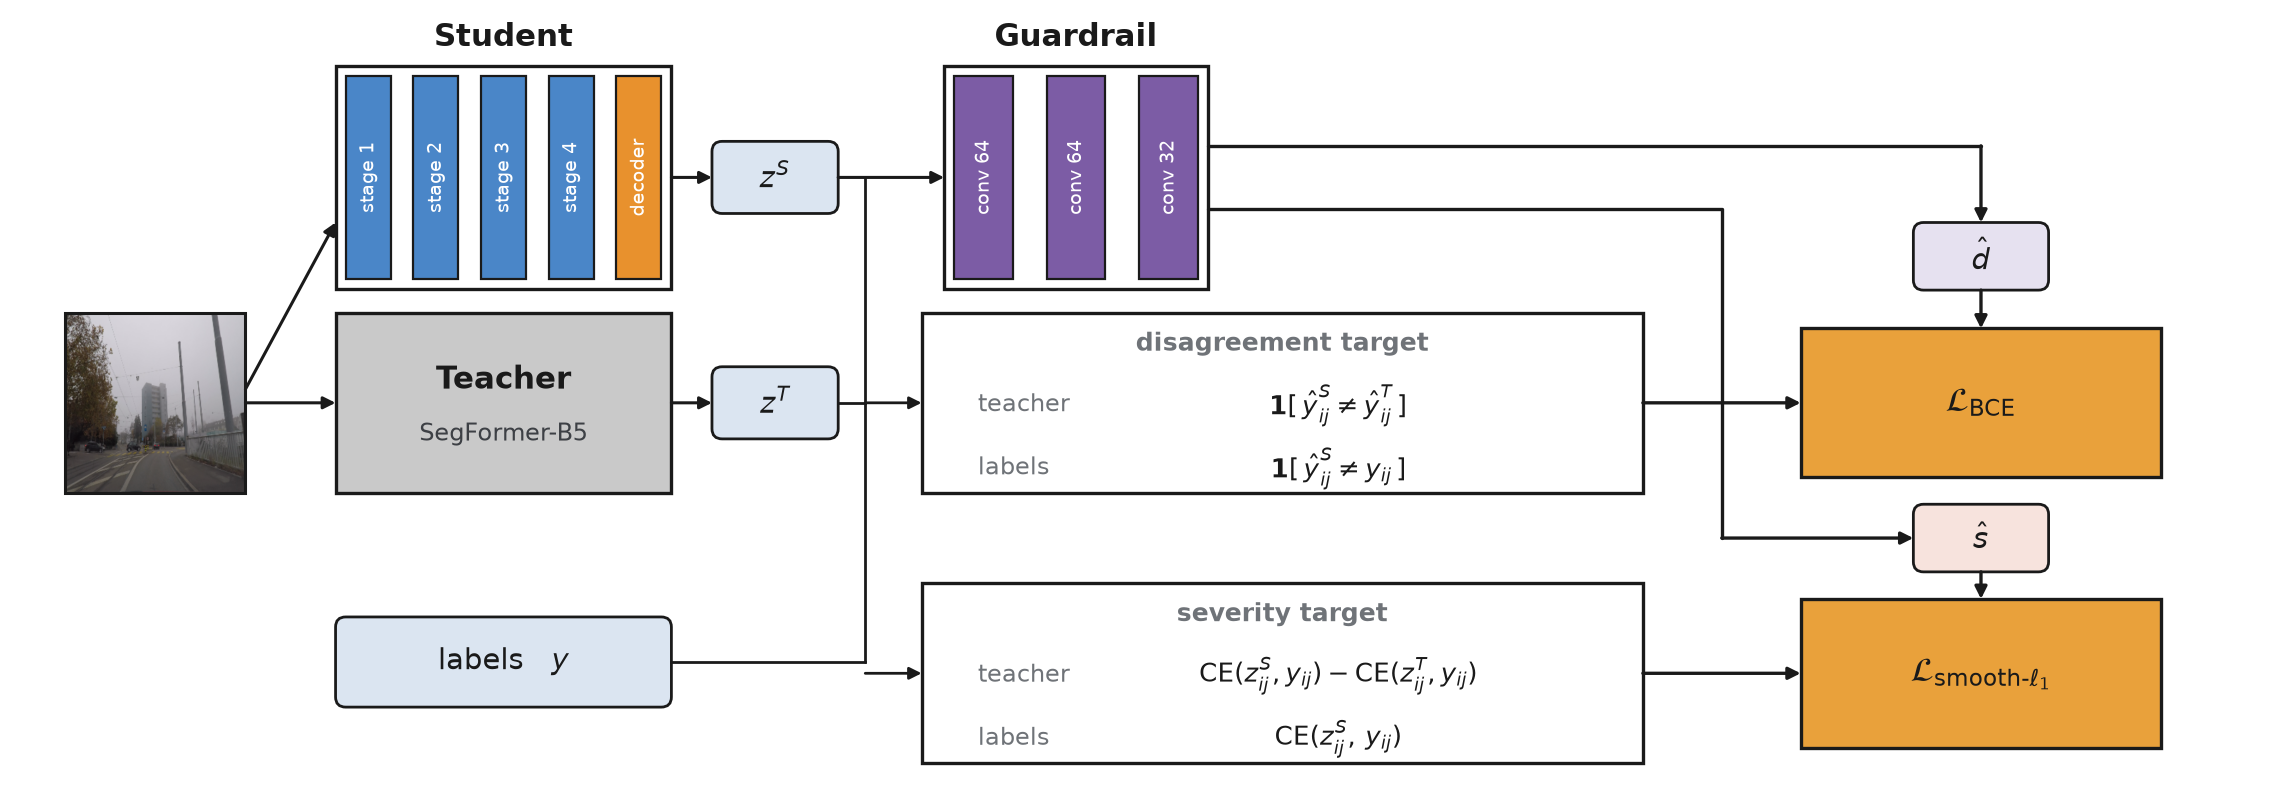
\includegraphics[width=\linewidth]{fig_arch_training.png}
\caption{Stage-4 guardrail training. The student and teacher are frozen; the two dense targets are formed either from the teacher's predictions and losses or from the labels, and everything else---head, optimizer, schedule, corruption policy---is held fixed between the two cases.}
\label{fig:arch-training}
\end{figure}


\paragraph{Inference.}
At test time the guardrail is used as a dense risk predictor rather than as a teacher simulator. Given an image $x$, it produces a per-pixel severity map $\hat s(x)$, which is pooled into a scalar image-level failure score
\[
g(x)
=
\sigma\!\left(
\frac{\sum_{ij} m_{ij} \hat s_{ij}(x)}{\sum_{ij} m_{ij}}
\right)
\in [0,1],
\]
where $\sigma(\cdot)$ is the sigmoid. Larger $g(x)$ means higher predicted failure risk. The same mask $m$ pools every image-level score in our comparison, including all post-hoc baselines, so it enters symmetrically and does not favour any method. We treat $g(x)$ as a ranking score for selective prediction, not as a calibrated probability of failure. The disagreement head is only used as an auxiliary training signal that shapes the shared encoder, so the default inference-time score is computed from the severity head alone. A threshold on $g(x)$ can flag high-risk inputs or trigger teacher deferral, and because $g(x)$ depends only on the frozen student logits and the lightweight head, inference is a single forward pass through $S$ and $G$ with no teacher invocation.

\begin{figure}[H]
\centering
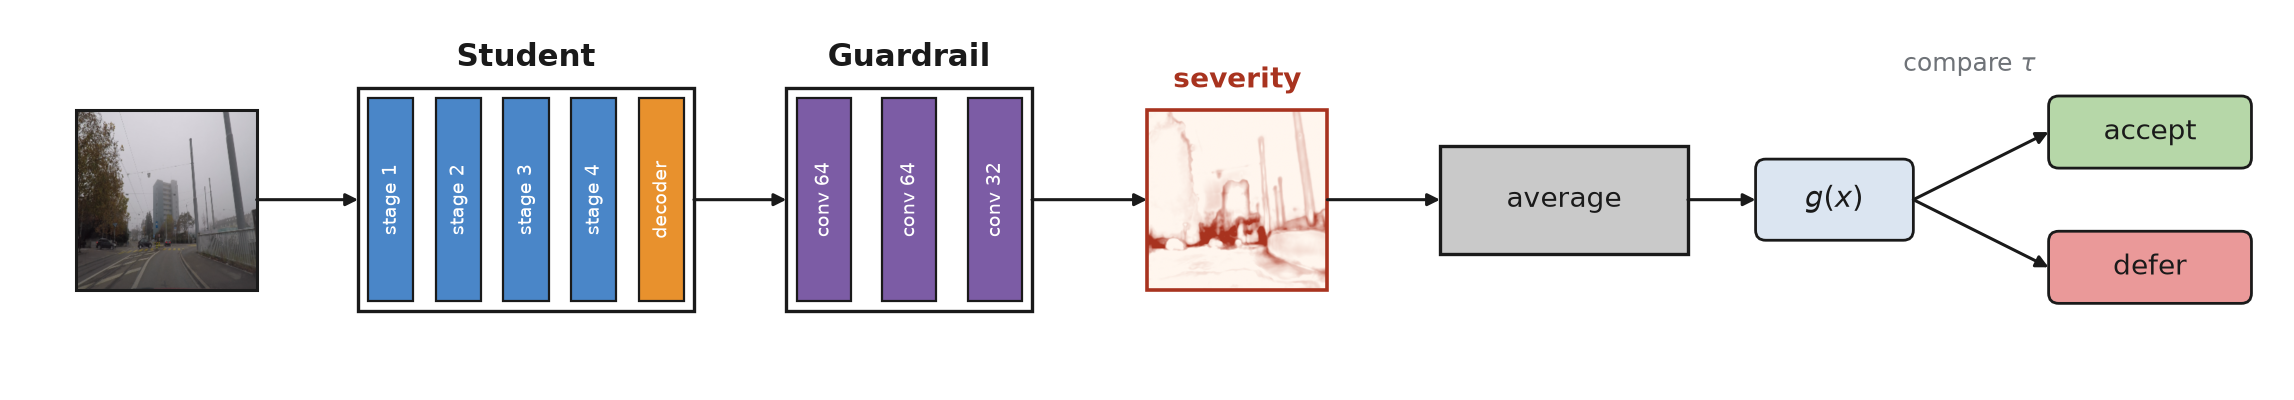
\includegraphics[width=\linewidth]{fig_arch_inference.png}
\caption{Inference. The severity map is mask-averaged into the scalar score $g(x)$, which is compared against an operating threshold to accept the student's prediction or defer.}
\label{fig:arch-inference}
\end{figure}


\paragraph{Guardrail $+$ post-hoc.}
Post-hoc scores such as energy and max-logit are fixed nonlinear functions of the student's logits, so they carry no information beyond $z^S$. Although $G$ already receives the logits and the student features, a shallow convolution struggles to recover these global logit-magnitude statistics on its own. We therefore introduce a variant that concatenates per-pixel energy and max-logit as two additional input channels to $G$. This widens the first layer's input, and the head, training procedure, and targets are otherwise unchanged.

\begin{figure}[H]
\centering
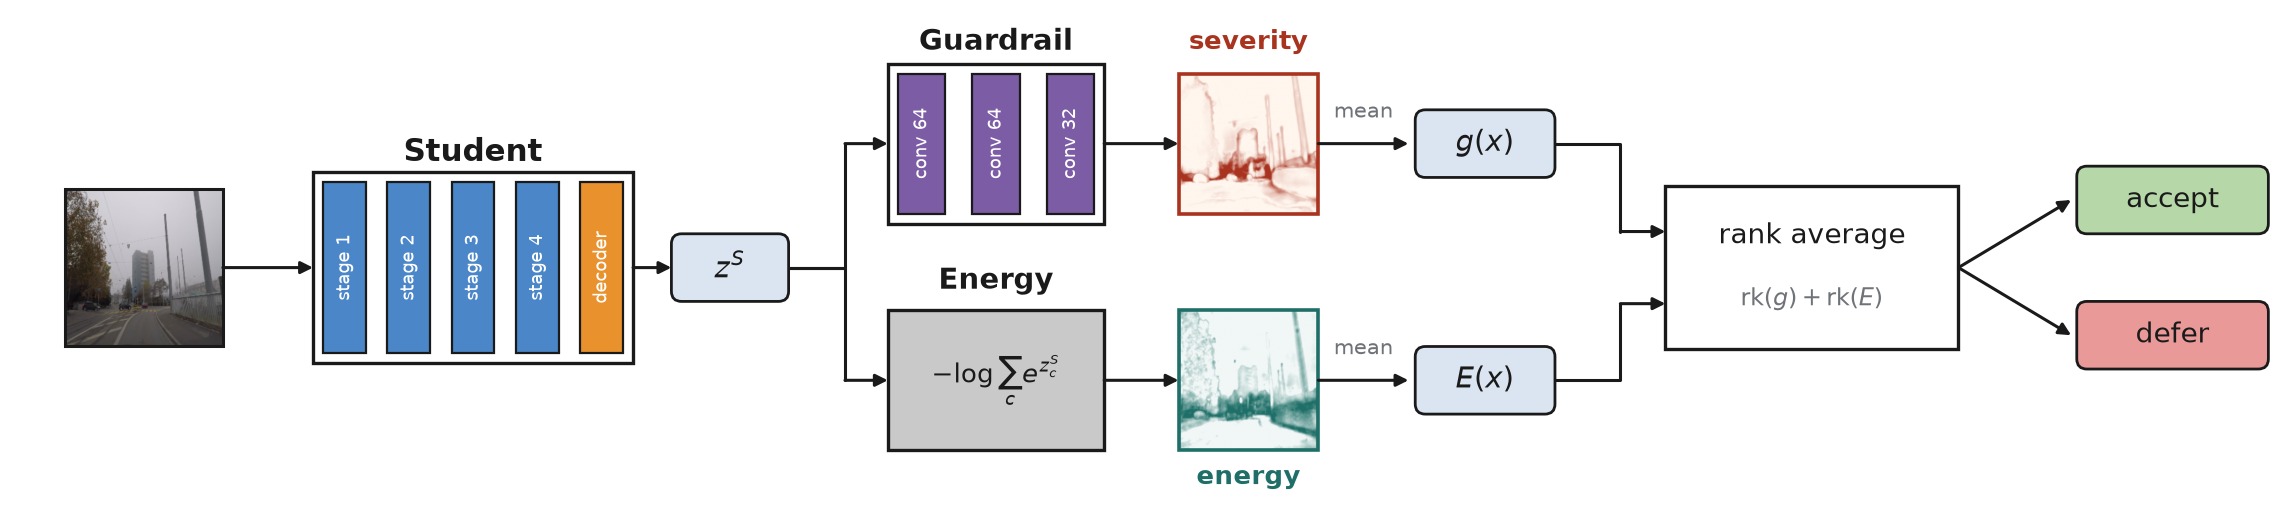
\includegraphics[width=\linewidth]{fig_arch_fusion.png}
\caption{Fusing the guardrail with a post-hoc magnitude score. The guardrail severity and the per-pixel energy are each mask-averaged and rank-averaged into a single selective score.}
\label{fig:arch-fusion}
\end{figure}


\paragraph{Teacher signal under shift.}

\begin{table}[H]
\centering
\small
\setlength{\tabcolsep}{5pt}
\caption{Breakdown of mIoU and the pixels where the student and teacher disagree (mit-b1). mIoU is the standard $19$-class macro average over the pooled dataset. The right-hand block splits the pixels where the student's and teacher's predicted classes differ, as a percentage of valid pixels, according to which model matches the ground truth; the three sub-columns partition \emph{Any}. We see the dominant case for out-of-distribution is the teacher advantage, which can be recovered with teacher labels for the guardrail. Percentages are means of per-image fractions.}
\label{tab:diag}
\begin{tabular}{lccrrrr}
\toprule
 & \multicolumn{2}{c}{mIoU} & \multicolumn{4}{c}{Disagreeing pixels (\% of valid pixels)} \\
\cmidrule(lr){2-3} \cmidrule(lr){4-7}
 & Student & Teacher & Any & Teacher right & Student right & Both wrong \\
\midrule
Cityscapes (in-domain) & .691 & .774 & 4.2 & 2.7 & 1.1 & 0.4 \\
ACDC (adverse conditions) & .405 & .517 & 16.6 & 9.4 & 2.4 & 4.7 \\
IDD (India) & .459 & .532 & 8.7 & 4.7 & 2.1 & 1.9 \\
BDD (US) & .445 & .554 & 10.6 & 6.7 & 2.1 & 1.9 \\
\bottomrule
\end{tabular}
\end{table}

It seems counterintuitive to train a reliability guardrail head on a teacher's predictions rather than the ground-truth labels; however, a ground-truth target considers all errors identical, while teacher errors are often artifacts of the image that no abstention or deferral can cover. A teacher target is only worth training on if the cases where the student errs while the teacher is correct are meaningful. Table~\ref{tab:diag} shows that this case---the teacher being right relative to the student---is abundant, and thus that there is room for student improvement to train the guardrail on. For in-domain cases the student--teacher disagreement is low and the guardrail should then be trained on ground-truth labels, but for out-of-distribution cases we see a significant gap of $4.7$--$9.4\%$ of valid pixels, showing the teacher target has room to improve the guardrail. There is still the case where the student is correct but the teacher is wrong, and we see this is much less frequent than the teacher-correct case, yet it still must be considered. The severity head thus considers the ground-truth labels, as it computes $\mathrm{CE}(z^S, y) - \mathrm{CE}(z^T, y)$, while the disagreement head ignores the labels.


\section{Experiments}

\paragraph{Datasets.}
We use Cityscapes-val ($500$ images)~\cite{cordts2016cityscapes} as the in-domain dataset, because it is the source domain every model is trained on and therefore fixes the reference point against which shift is measured. ACDC-val ($406$ images)~\cite{sakaridis2021acdc} consists of fog, night, rain, and snow categories and fixes the geometry while varying the conditions, isolating adverse-condition shift. Additionally, IDD-val ($978$ images)~\cite{varma2019idd} and BDD100K-val ($1000$ images)~\cite{yu2020bdd100k} instead vary the scene itself, including road layout, traffic composition, and geography, to test whether the guardrail generalizes to the overall problem. All models are trained on Cityscapes only.

\paragraph{Baselines.}
We compare against MSP~\cite{hendrycks2017baseline}, temperature-scaled MSP~\cite{guo2017calibration}, MC-Dropout~\cite{gal2016dropout}, MaxLogit~\cite{hendrycks2022scaling}, entropy, the energy score~\cite{liu2020energy}, and Deep Ensembles~\cite{lakshminarayanan2017deepensembles}. Each baseline reduces the dense per-pixel score to an image-level score by averaging over the same valid pixels as $g(x)$. MC-Dropout ($4$ passes) and the three-member Deep Ensemble use predictive entropy of the mean softmax, and temperature scaling uses a fixed $T{=}2$. Exact per-baseline definitions, sign conventions, and dataset/label-mapping details are in Appendix~\ref{app:impl}. Multi-task is the default unless stated otherwise. Our controlled comparison of teacher vs.\ ground-truth supervision uses the SegFormer-b1 student trained on three seeds ($42/137/256$) and averaged over them, so the teacher-vs-GT differences are matched seed-for-seed. Confidence-feature results (\S\ref{sec:conffeat}) use five seeds across three backbones (b0/b1/b2).

\paragraph{Metrics.}
We consider per-image quality as mIoU: the mean IoU over the classes that appear in the union of the ground truth and the predictions, computed over valid pixels only. We label an image a failure if $\rho = 1 - \mathrm{mIoU}$ is in the worst $20\%$ of the images scored. This is a relative ranking rather than an absolute correctness ranking, the cutoff is evaluated retrospectively rather than at a deployable threshold, and an equally poor image in a uniformly hard dataset may fall outside of this quintile. We therefore read out numbers as a failure-ranking benchmark. For IDD and BDD we read the $80$th-percentile cutoff as a single global value over the dataset, while for ACDC it is computed separately within each condition and applied to the pooled set, so one uniformly difficult split does not dominate the failure set. F-AUROC ranks a score against this label over all images, and confident-failure AUROC (CF-AUROC) restricts the ranking to the confident subset with image-level MSP $\geq \tau$, where the image-level MSP is the mean over valid pixels of the per-pixel maximum softmax probability, for $\tau \in \{0.85, 0.95, 0.97\}$. CF-AUROC finds, among images the deployed student considers confident, which score best ranks the failures. Part of MSP's decline at large $\tau$ is a consequence of conditioning on MSP. We only depart from the per-condition ACDC cutoff in \S\ref{sec:within-condition}, because the purpose there is to measure the between-condition signal that a per-condition cutoff removes. Under that global cutoff, night accounts for almost all failures.


\section{Results}

\subsection{Comparison with post-hoc methods}
\label{sec:teacher-vs-gt}

We compare with post-hoc metrics; Table~\ref{tab:main} reports CF-AUROC @ $\tau = 0.85$.

\begin{table}[H]
\centering
\small
\setlength{\tabcolsep}{3pt}
\caption{CF-AUROC @ MSP$\,{\geq}\,$0.85 (mit-b1), a near-full-coverage operating point (retained images: ACDC $397/406$, IDD $976/978$, BDD $987/1000$), evaluated over three training seeds ($42/137/256$) with low per-seed variation (std $\leq.007$ for every head and dataset). GT heads use the same architecture and training as the teacher heads; only the supervision source differs. DeepEns is a single three-member ensemble (no seed averaging), scored on the same full validation splits as every other cell.}
\label{tab:main}
\begin{tabular}{lcccccccccc}
\toprule
 & MSP & Ent & MaxL & Energy & MC-D & DeepEns & GT-Dis & GT-Gap & \textbf{T-Multi} & $\Delta_{\text{GT}}$ \\
\midrule
ACDC & .587 & .592 & .596 & .594 & .593 & \win{.605} & .587 & .595 & \win{.605} & \win{+1.0} \\
IDD & .573 & .578 & .543 & .539 & .577 & .590 & .570 & .595 & \win{.607} & \win{+1.2} \\
BDD & .657 & .680 & .732 & .730 & .682 & .723 & .731 & .722 & \win{.765} & \win{+3.5} \\
\bottomrule
\end{tabular}
\end{table}

Table~\ref{tab:main} is the controlled experiment for the supervision signal, as T-Multi, GT-Gap, and GT-Dis share the same architecture, optimizer, and seeds, so $\Delta_{\mathrm{GT}}$ attributes the difference to the target alone. T-Multi is the strongest score on all three datasets, matching a three-member Deep Ensemble on ACDC and beating it on IDD and BDD without training or deploying two extra students. The margins over the best ground-truth head are small on ACDC and IDD but larger on BDD, though absolute values near $0.6$ suggest that ranking confident failures under shift is far from solved. The table thus shows that for the same head and no teacher call at test time, a teacher-relative dense target is a stronger learning signal than ground-truth correctness on out-of-distribution data.

\begin{figure}[H]
\centering
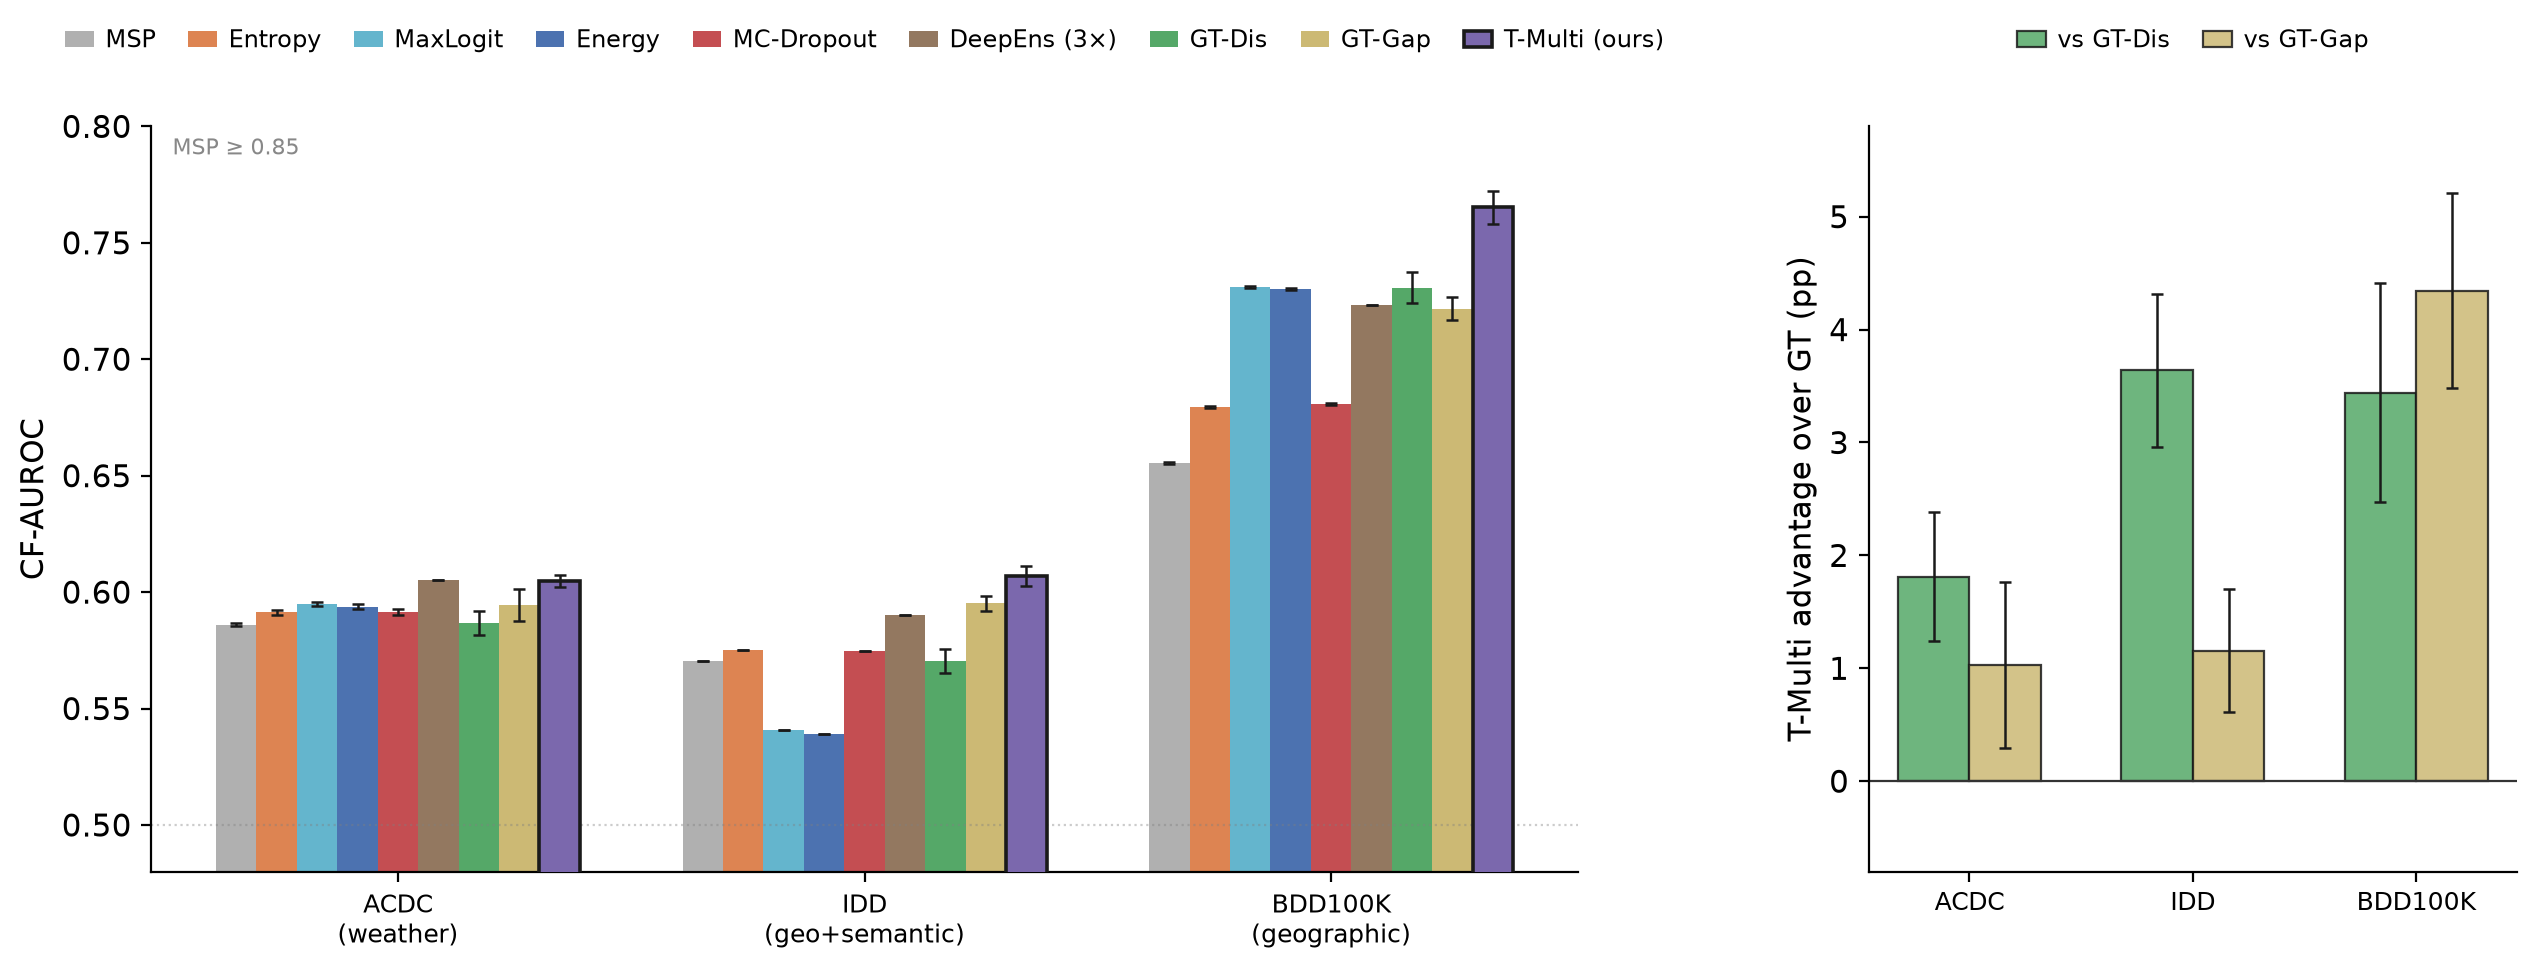
\includegraphics[width=\linewidth]{fig_teacher_vs_gt.png}
\caption{Left: CF-AUROC @ MSP$\,{\geq}\,$0.85 across methods and datasets (mit-b1). Right: T-Multi improvement over each GT baseline in percentage points. Error bars are $\pm1$ std.}
\label{fig:main}
\end{figure}

We see the spread between the best and worst detector widens with the type of shift, with roughly $2$\,pp on ACDC, $7$ on IDD, and $11$ on BDD. So the choice of scoring method is slight for near-distribution cases such as ACDC and decisive under geographic shift. No post-hoc score is strong on all three datasets: MaxLogit is the strongest baseline on BDD, yet is the weakest by $2.7$\,pp compared to GT-Dis on IDD. The right panel shows the fragility of the supervision target itself, as GT-Gap performs better over ACDC and IDD while GT-Dis performs better on BDD, so $\Delta_{\mathrm{GT}}$ shows that neither of the two is reliably the runner-up. T-Multi is the strongest on all three datasets, and the teacher-vs-GT gap can be tested directly across seeds, where T-Multi beats the better of the two GT heads in every cell ($\Delta{=}{+}0.019$; two-sided sign test $p{=}0.004$). Per-seed spread is small, so these orderings reflect the supervision signal rather than noise.

\paragraph{Paired-image bootstrap.}
A complementary paired-image bootstrap ($N{=}3000$ resamples with replacement within each dataset, at seed $42$) attributes the T-Multi vs.\ GT-Dis advantage to BDD ($\Delta{=}{+}0.021$, $p{=}0.007$) and IDD ($\Delta{=}{+}0.030$, $p{<}0.001$), with no significance on ACDC ($\Delta{=}{+}0.014$, $p{=}0.23$). Pooled, we find $+0.022$ ($p{=}0.010$) over GT-Dis and $+0.020$ ($p{=}0.040$) over GT-Gap. This pattern agrees with the within-condition analysis (\S\ref{sec:within-condition}) in showing that the ACDC gains primarily come from condition-level separation rather than within-condition ranking.


\subsection{High-confidence failure detection}

Increasing $\tau$ does not simply make the task harder. Conditioning on MSP $\geq \tau$ removes the cases MSP as a confidence score would have removed. This leaves the failures MSP cannot rank, which the guardrail is designed to target.

\begin{table}[H]
\centering
\small
\setlength{\tabcolsep}{3pt}
\caption{CF-AUROC at strict thresholds (mit-b1). Probabilistic post-hoc scores decay as $\tau$ rises, compared to magnitude-based scores which are more resilient on IDD though not on BDD. $n$ is the number of confident images at each threshold. GT-Dis, GT-Gap and T-Multi entries are means over the same three seeds ($42/137/256$); seed variation grows as the confident subset shrinks (std $\leq.008$ for $\tau\leq0.90$, up to $.016$ at $0.95$ and $.051$ at $0.97$). DeepEns is a single three-member ensemble (no seed averaging) scored on the same full validation splits. ACDC is reported to $\tau{=}0.90$: its confident subset shrinks far faster than the others ($144$ images at $0.95$, $23$ at $0.97$, against $622$ and $169$ for BDD).}
\label{tab:strict}
\begin{tabular}{llrcccccccc}
\toprule
 & $\tau$ & $n$ & MSP & MaxL & Energy & MC-D & DeepEns & GT-Dis & GT-Gap & \textbf{T-Multi} \\
\midrule
\multirow{2}{*}{ACDC}
 & 0.85 & 397 & \loss{.586} & .595 & .594 & .592 & \win{.605} & .587 & .595 & \win{.605} \\
 & 0.90 & 364 & \loss{.559} & .569 & .568 & .563 & .575 & .564 & .577 & \win{.586} \\
\midrule
\multirow{4}{*}{IDD}
 & 0.85 & 976 & .570 & .541 & \loss{.539} & .575 & .590 & .570 & .595 & \win{.607} \\
 & 0.90 & 959 & .564 & .535 & \loss{.533} & .569 & .583 & .565 & .592 & \win{.603} \\
 & 0.95 & 634 & \loss{.501} & .505 & .505 & .509 & .524 & .502 & .524 & \win{.547} \\
 & 0.97 & 231 & .485 & \win{.564} & \win{.564} & .498 & .498 & .488 & .515 & \loss{.471} \\
\midrule
\multirow{4}{*}{BDD}
 & 0.85 & 987 & \loss{.655} & .731 & .730 & .681 & .723 & .731 & .722 & \win{.765} \\
 & 0.90 & 959 & \loss{.607} & .695 & .694 & .635 & .684 & .683 & .677 & \win{.726} \\
 & 0.95 & 622 & \loss{.487} & .592 & .592 & .531 & .601 & .600 & .582 & \win{.673} \\
 & 0.97 & 169 & \loss{.341} & .380 & .380 & .395 & .471 & .412 & .453 & \win{.566} \\
\bottomrule
\end{tabular}
\end{table}

After $\tau{=}0.95$, multiple scores fall below chance, where MSP reaches $0.341$, meaning that inside the subset of confident scores a higher score is associated with higher risk---the silent failure case. This is not due to conditioning on MSP: taking the BDD $\tau{=}0.97$ subset of $n{=}169$ and, rather than ordering by MSP, ordering by MaxLogit, Energy, or the guardrail leaves MSP at $0.306$, $0.323$, and $0.263$ respectively, so self-selection may even flatten MSP by ${\sim}4$\,pp. Against BDD at $\tau{=}0.97$, T-Multi is the only method to score above chance, and its margin over the better GT head grows monotonically. IDD inverts at $\tau{=}0.97$, where T-Multi falls to $0.471$ while MaxLogit and Energy reach $0.564$, which holds across three seeds ($+13.8$, $+7.4$, $+6.5$\,pp) and a paired-image bootstrap ($\Delta{=}{+}13.8$\,pp at seed $42$, $95\%$ CI $[+4.7,+23.4]$, $p{=}0.003$). The cause is a degeneracy in the head rather than a strength of the baselines: on IDD, the standard deviation of the guardrail score contracts $3.8\times$ between $\tau{=}0.85$ and $0.97$ ($.0139$ to $.0037$) while the risk it ranks keeps its spread ($.078$ to $.076$). This leaves it four times flatter than the same head on BDD at the same threshold ($.0145$). The contraction tracks the training signal: inside IDD's confident subset, the ratio of recoverable to misleading disagreement pixels falls to $1.75$ compared to $2.68$ on BDD, so the teacher-relative target the head was trained to predict is almost absent where it ranks. This is distinct from the night weakness (\S\ref{sec:within-condition}), where the risk is nearly constant and there is little to detect, compared to this case where the risk varies normally but the detector's predictions are more constant. We only consider subset sizes $\geq 150$ samples (Hanley--McNeil standard error of $0.06$), as reliability at the strict end is bounded by subset size rather than training variance.

\begin{figure}[H]
\centering
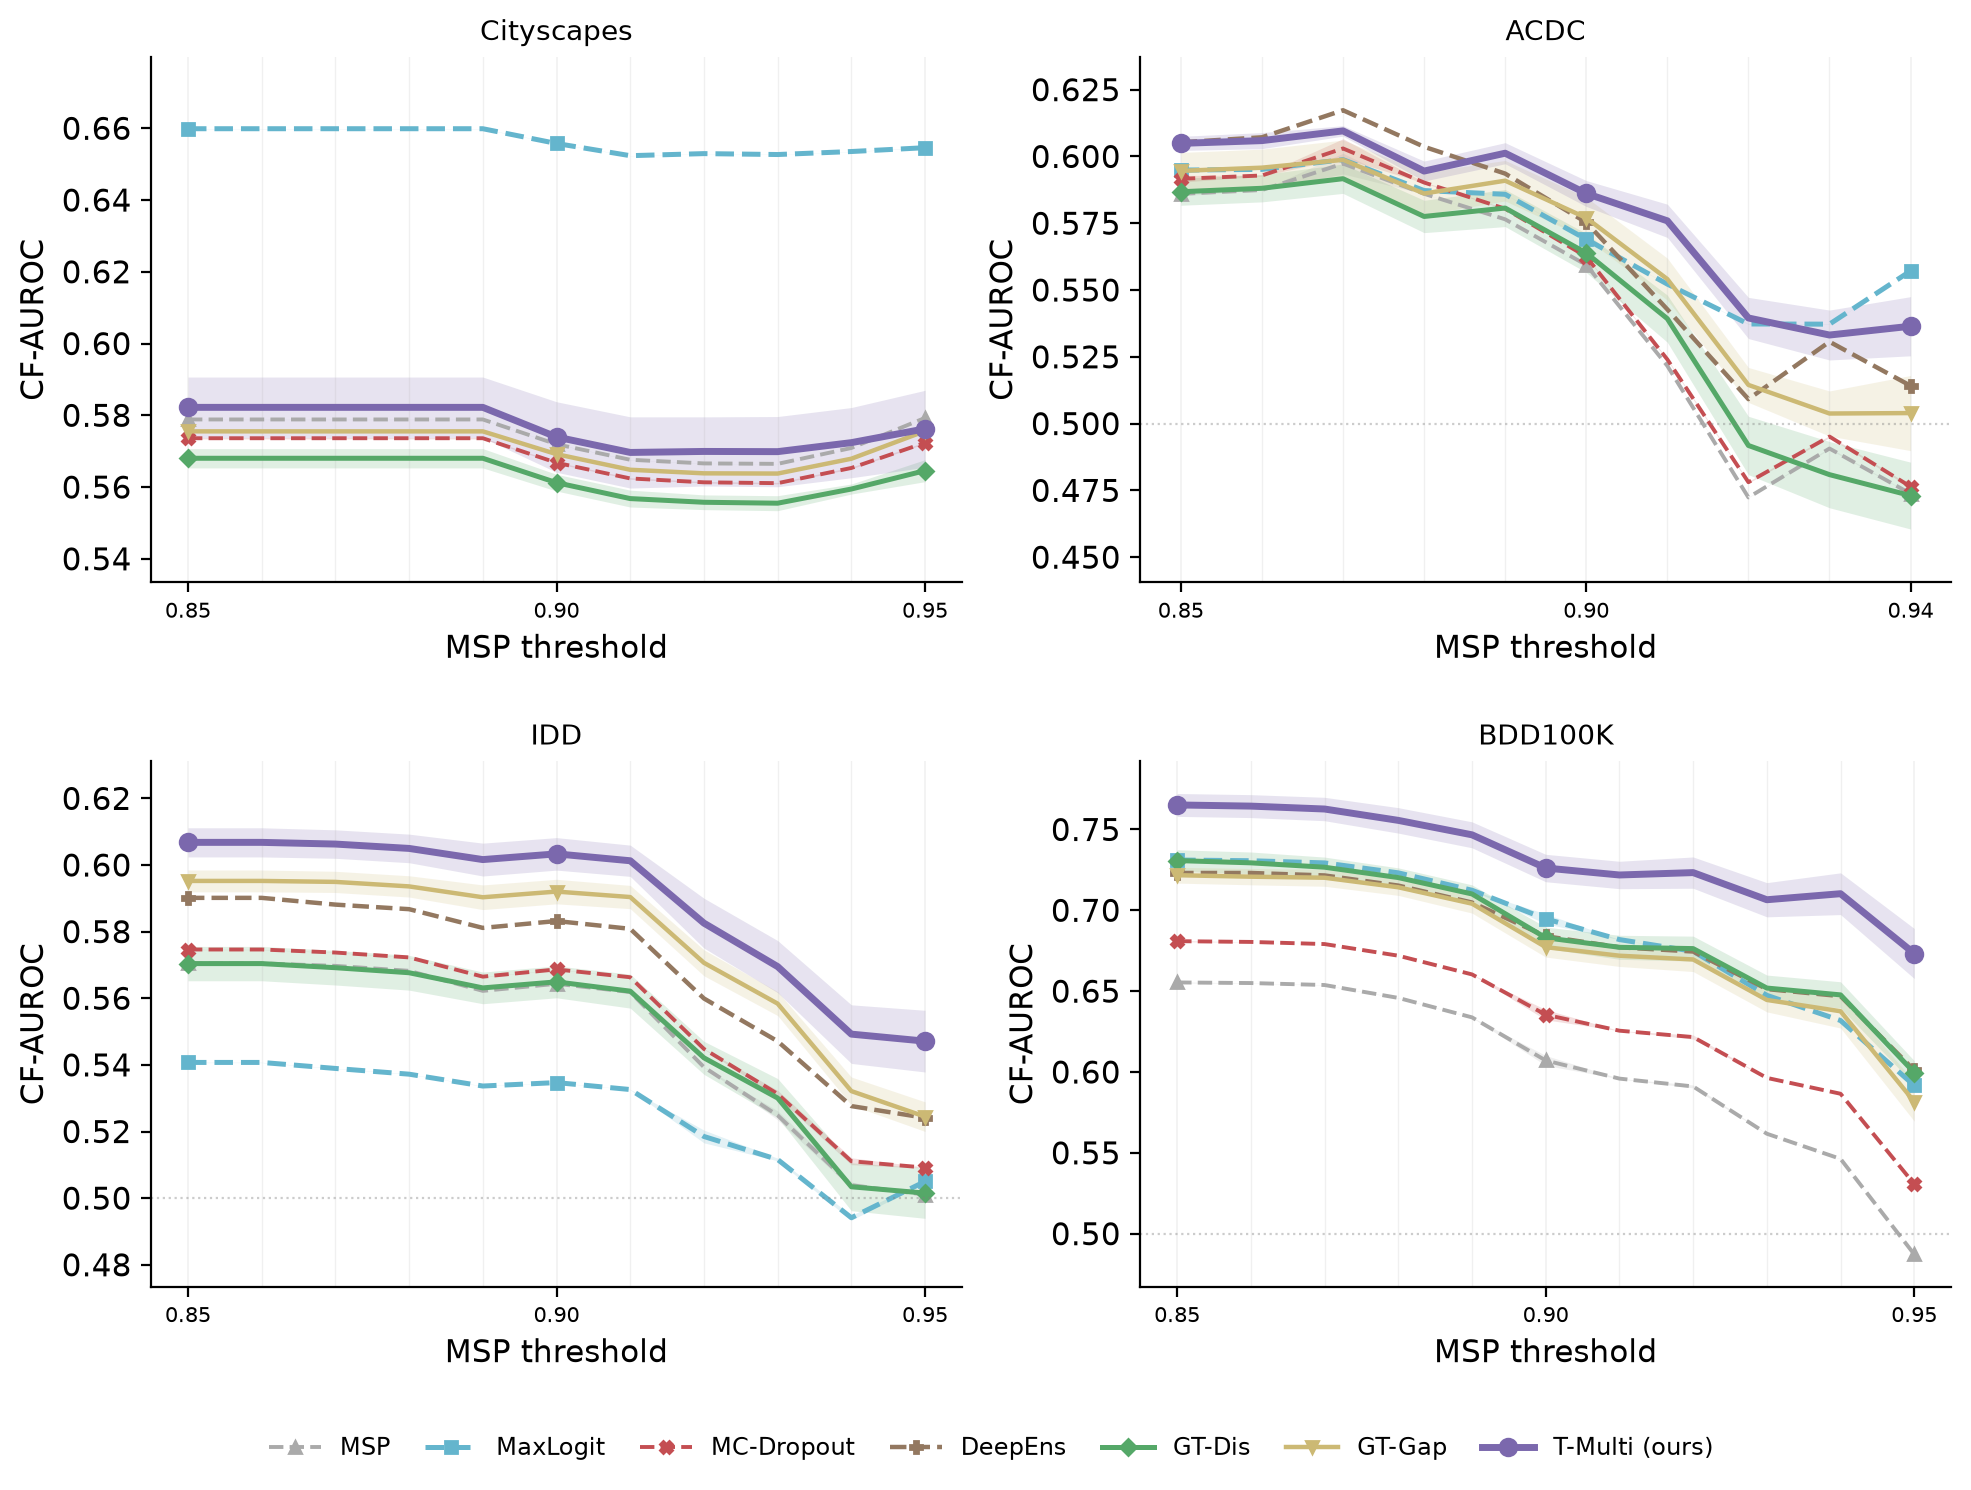
\includegraphics[width=\linewidth]{fig_threshold_sweep.png}
\caption{CF-AUROC swept at $0.01$ steps (mit-b1). Lines are seed means with $\pm 1$ std shaded. A threshold is plotted only where the dataset retains at least $150$ confident images, which truncates ACDC to $\tau{=}0.94$.}
\label{fig:sweep}
\end{figure}

We sweep $\tau$ to confirm Table~\ref{tab:strict} is not a lucky sample: T-Multi leads over all $11$ BDD and IDD thresholds, while on ACDC no method consistently wins, though every gap between T-Multi and the best alternative is $\leq 2.2$\,pp across all thresholds. Cityscapes shows the limitations, as the guardrail does not perform better in-domain, while MaxLogit clearly wins. In-domain, confident errors are visible in the student's logit magnitudes, so a post-hoc score suffices and a learned head adds nothing. Under shift the post-hoc methods struggle to track risk, and a teacher-supervised guardrail performs better as shift increases.


\subsection{Within-condition analysis}
\label{sec:within-condition}

\begin{table}[H]
\centering
\small
\setlength{\tabcolsep}{4pt}
\caption{Within-condition failure AUROC (ACDC, mit-b1). The per-condition rows and their macro-average use a \emph{balanced} per-condition failure cutoff (worst $20\%$ within each condition). The pooled and condition-only rows instead use a single \emph{global} ACDC cutoff, under which failures concentrate in night. Condition-only assigns each image its condition's mean risk.}
\label{tab:within}
\begin{tabular}{lcccccc}
\toprule
Cond. & MSP & MaxL & MC-D & GT-Dis & GT-Gap & \textbf{T-Multi} \\
\midrule
Fog & .495 & .576 & .503 & .519 & .521 & \win{.600} \\
Night & .607 & \win{.760} & .625 & .670 & .659 & .590 \\
Rain & .734 & .628 & .749 & .747 & .762 & \win{.764} \\
Snow & .552 & \win{.664} & .554 & .602 & .628 & .636 \\
\midrule
Macro-avg & .597 & \win{.657} & .608 & .634 & .643 & .648 \\
\midrule
Condition-only & \multicolumn{6}{c}{$0.932$ (assigns condition mean risk, global cutoff)} \\
Pooled & .692 & .927 & .710 & .910 & .903 & \win{.928} \\
\bottomrule
\end{tabular}
\end{table}

\begin{figure}[H]
\centering
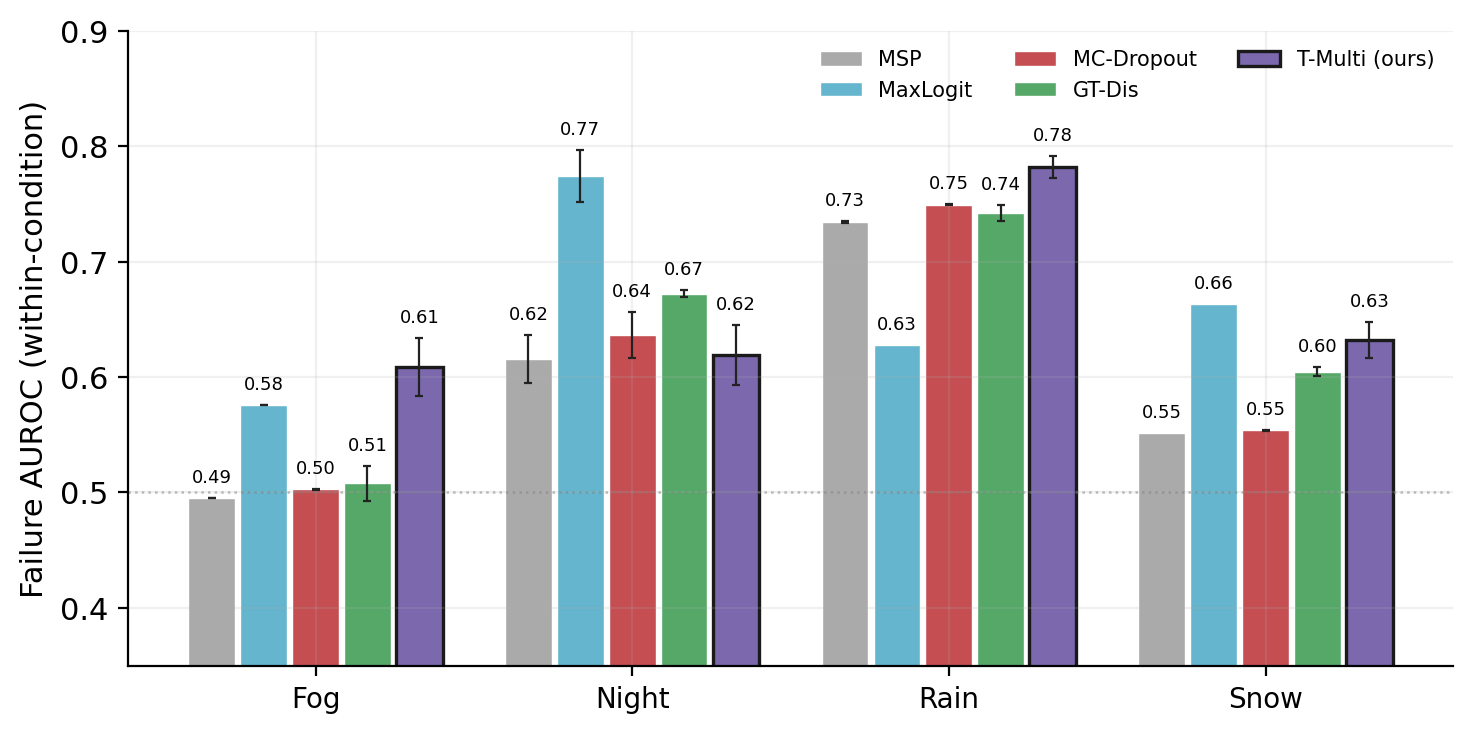
\includegraphics[width=0.9\linewidth]{fig_within_condition.png}
\caption{Within-condition failure AUROC on ACDC (mit-b1).}
\label{fig:within}
\end{figure}


\subsection{Supervision mode ablation}

\begin{table}[H]
\centering
\small
\setlength{\tabcolsep}{4pt}
\caption{Full ablation of supervision modes (b1, CF-AUROC @ MSP$\,{\geq}\,$0.85). All six modes are compared at the single matched seed $42$, since Scalar, T-Dis and T-Gap were trained at that seed only; the three-seed means for GT-Dis, GT-Gap and T-Multi are in Table~\ref{tab:main}.}
\label{tab:ablation}
\begin{tabular}{lccccccc}
\toprule
 & MSP & Scalar & GT-Dis & GT-Gap & T-Dis & T-Gap & T-Multi \\
\midrule
City & .579 & .613 & .566 & .576 & .574 & .583 & .571 \\
ACDC & .587 & .569 & .589 & .599 & .582 & .597 & \win{.604} \\
IDD & .573 & .570 & .575 & .592 & .585 & .617 & .603 \\
BDD & .657 & .754 & .738 & .716 & .745 & .747 & \win{.758} \\
\bottomrule
\end{tabular}
\end{table}


\paragraph{Scalar baseline.}\mbox{}

\begin{figure}[H]
\centering
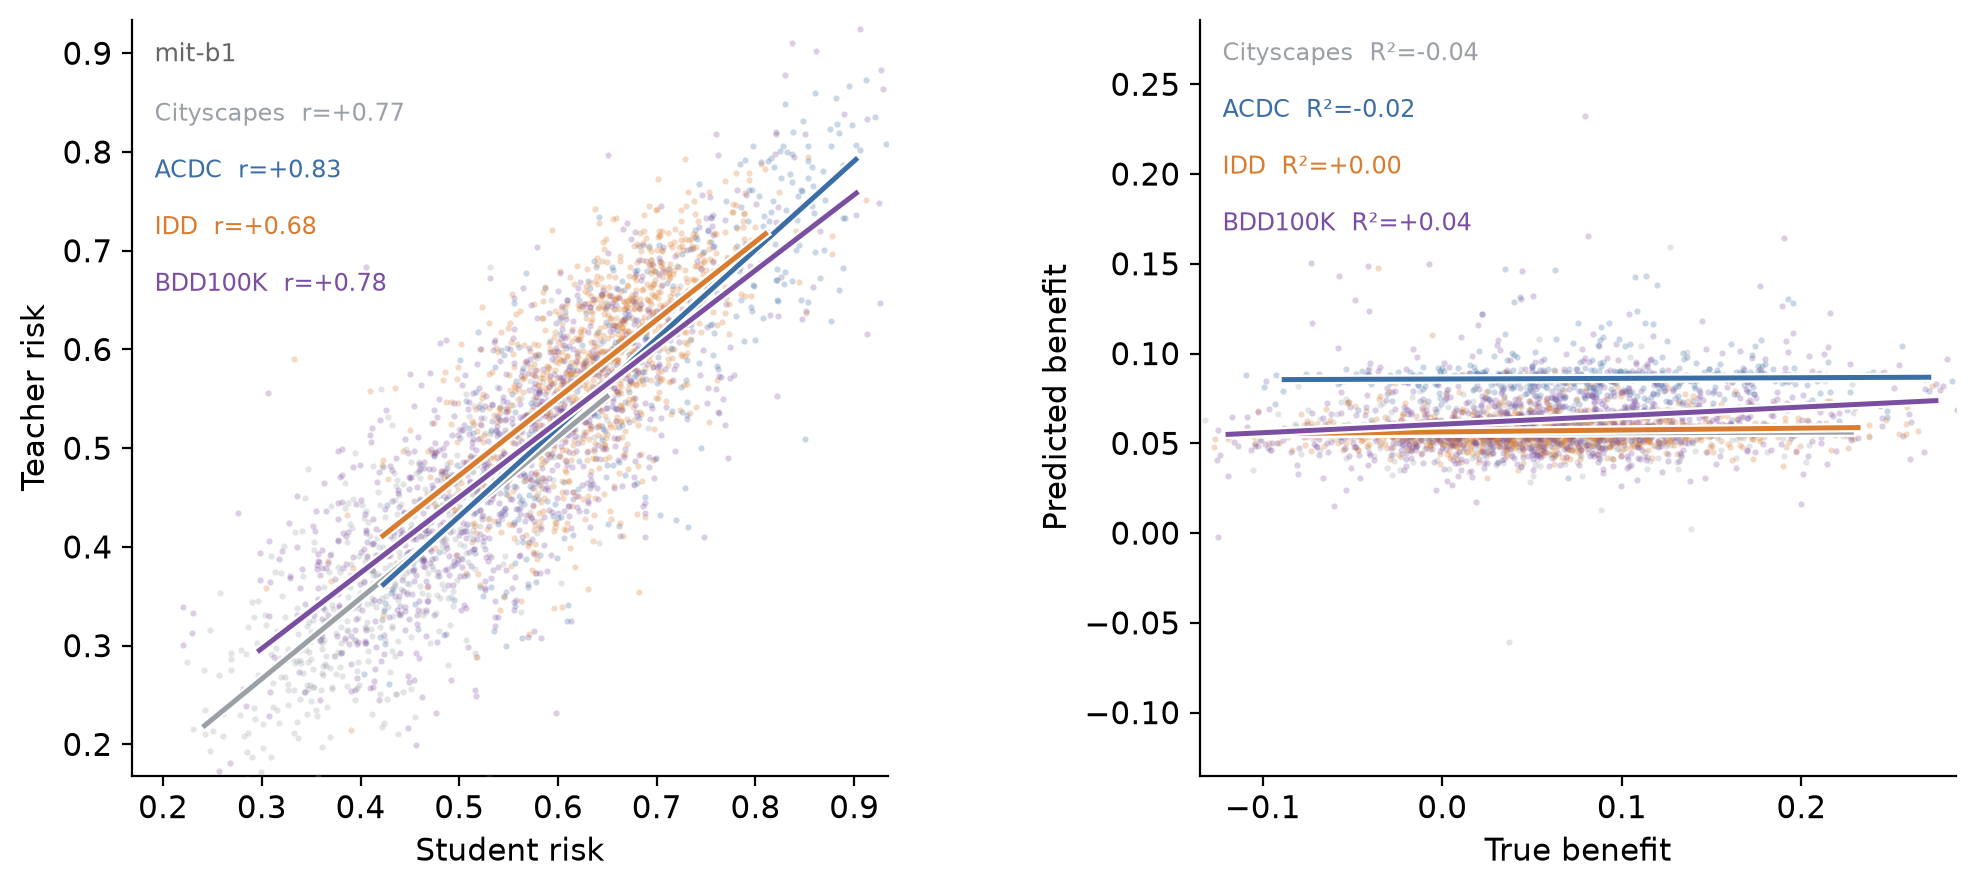
\includegraphics[width=\linewidth]{fig_negative_result_decomp.png}
\caption{Student and teacher risks are tightly coupled, so the per-image benefit is a thin residual that cannot be recovered from the student's logits ($R^2 \leq 0.04$ out-of-fold, right), motivating the dense per-pixel supervision.}
\label{fig:scalar}
\end{figure}


\subsection{Confidence features}
\label{sec:conffeat}

\begin{table}[H]
\centering
\small
\setlength{\tabcolsep}{6pt}
\caption{Confidence-feature head vs.\ the energy score (CF-AUROC @ MSP$\,{\geq}\,$0.85 on ACDC). Per-backbone columns are means over five seeds; the energy score has no learned parameters, so it is identical across seeds and its only variation is between backbones. Pooled is the mean over all $3{\times}5{=}15$ guardrail runs.}
\label{tab:conffeat}
\begin{tabular}{lcccc}
\toprule
Method & b0 & b1 & b2 & Pooled \\
\midrule
Energy score & .590 & .595 & .582 & .589\,{\scriptsize$\pm$.005} \\
Guardrail $+$ conf.\ features (ours) & \win{.624} & \win{.620} & \win{.589} & \win{.611\,{\scriptsize$\pm$.017}} \\
\midrule
$\Delta$ vs.\ energy & \win{+3.4} & \win{+2.5} & \win{+0.7} & \win{+2.2} \\
\bottomrule
\end{tabular}
\end{table}


\subsection{Inference cost and reliability comparison}
\label{sec:latency}

\begin{table}[H]
\centering
\small
\setlength{\tabcolsep}{6pt}
\caption{Per-image inference latency vs.\ confident-failure AUROC at MSP$\,\geq 0.95$ on three datasets (mit-b1, 1$\times$NVIDIA L40S, batch size $=4$). ACDC is the per-condition mean over fog/night/rain/snow. Latencies are medians over $500$ Cityscapes-val images after $50$ warm-up passes, with CUDA synchronization on each forward pass. The teacher row reports latency only: it is the deferral target rather than a scorer, so it has no confident-failure AUROC.}
\label{tab:latency-auroc}
\begin{tabular}{lccccc}
\toprule
Method & Latency (ms) & ACDC & IDD & BDD100K & Mean OOD \\
\midrule
Student (MSP) & 4.9 & .437 & .501 & .487 & .475 \\
MaxLogit & 4.9 & .534 & .505 & .589 & .543 \\
MC-Dropout (4 passes) & 25.2 & .432 & .509 & .530 & .490 \\
Student + guardrail (T-Multi, ours) & 16.8 & .573 & .548 & .673 & .598 \\
Teacher (full inference) & 26.1 & --- & --- & --- & --- \\
\bottomrule
\end{tabular}
\end{table}

\paragraph{Pareto analysis.}\mbox{}

\paragraph{Selective deferral.}\mbox{}

\begin{table}[H]
\centering
\small
\setlength{\tabcolsep}{6pt}
\caption{Teacher-deferral benefit vs.\ cost (mit-b1). Each detector routes its highest-risk fraction $f$ of frames to the teacher; entries are the percentage of total student$\to$teacher mIoU benefit recovered, pooled as the mean over ACDC/IDD/BDD of each dataset's percentage. Oracle ranks frames by the true per-frame student$\to$teacher mIoU benefit. Per-frame latency is method-specific: the post-hoc gates omit the $11.9$\,ms guardrail head, $\mathbb{E}[L]^{\text{post}}\!=\!4.9 + f\,{\cdot}\,26.1$\,ms, while the guardrail gate pays it, $\mathbb{E}[L]^{\text{guard}}\!=\!16.8 + f\,{\cdot}\,26.1$\,ms. Best non-oracle detector per row in bold.}
\label{tab:defer}
\begin{tabular}{lcccccccc}
\toprule
$f$ & $\mathbb{E}[L]^{\text{post}}$ & $\mathbb{E}[L]^{\text{guard}}$ & Random & MSP & MaxL & Energy & T-Multi & Oracle \\
\midrule
0.05 & 6.2 & 18.1 & 5.0 & 5.7 & \win{6.8} & \win{6.8} & 6.3 & 15.7 \\
0.10 & 7.5 & 19.4 & 10.0 & \win{13.0} & 12.9 & 12.9 & 12.6 & 27.9 \\
0.20 & 10.1 & 22.0 & 20.0 & 23.9 & \win{24.5} & 24.3 & 24.2 & 47.3 \\
\bottomrule
\end{tabular}
\end{table}

\paragraph{Selective prediction.}\mbox{}

\begin{figure}[H]
\centering
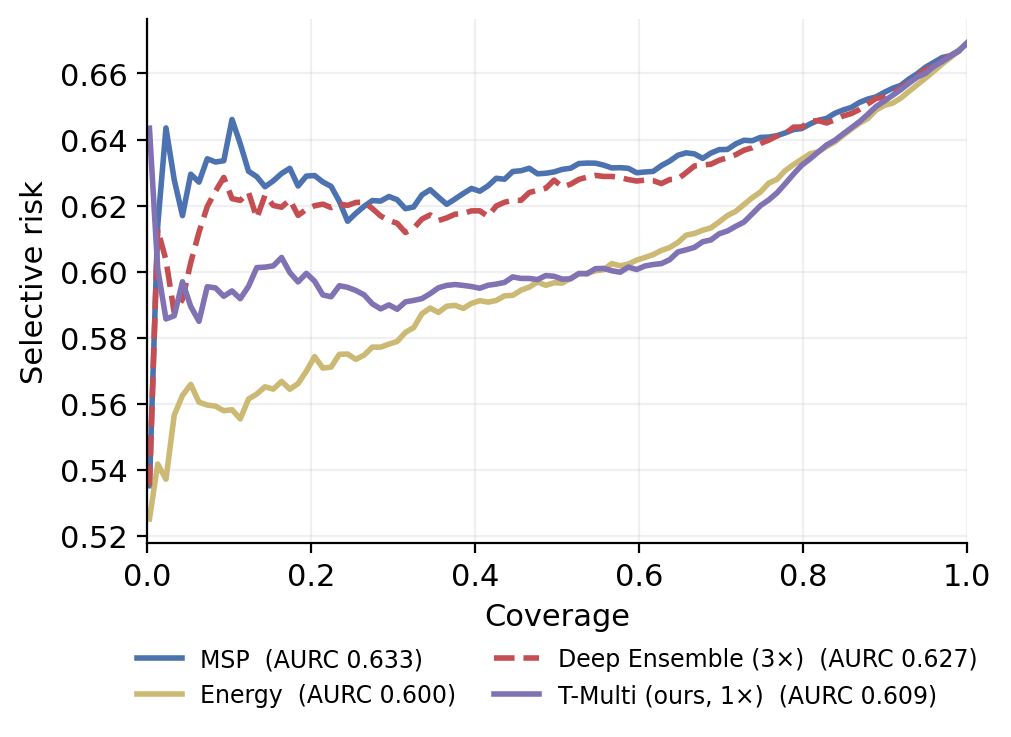
\includegraphics[width=0.62\linewidth]{fig_deep_ensemble.png}
\caption{Risk-coverage on ACDC (mit-b1). The single-pass guardrail (T-Multi) has lower overall selective risk (AURC $.609$ vs.\ $.627$) than the three-member Deep Ensemble, although the curves cross at low coverage. The post-hoc energy score is comparably strong.}
\label{fig:deepens-rc}
\end{figure}

\begin{table}[H]
\centering
\small
\setlength{\tabcolsep}{4pt}
\caption{AURC on mit-b1, seed $42$ (lower is better; images ranked by each score). AURC is the area under the risk-coverage curve: at coverage $c$ the selective risk is the mean per-image risk ($1-\mathrm{mIoU}$) of the most-confident $c$ fraction of images, integrated over $c\in(0,1]$ by the trapezoid rule (Appendix~\ref{app:impl}). This is the conventional AURC, not the generalized AUGRC of \citet{traub2024overcoming}. The three-member Deep Ensemble (Fig.~\ref{fig:deepens-rc}) has AURC $.627$ on ACDC, above every score here.}
\label{tab:augrc}
\begin{tabular}{lcccccccc}
\toprule
 & MSP & MaxL & Energy & TempMSP & MC-D & GT-Dis & GT-Gap & \textbf{T-Multi} \\
\midrule
City & .422 & \win{.415} & \win{.415} & .422 & .422 & .423 & .422 & .422 \\
ACDC & .634 & \win{.601} & .600 & .625 & .630 & .610 & .612 & .609 \\
IDD & .633 & .636 & .636 & .635 & \win{.632} & .634 & \win{.632} & \win{.632} \\
BDD & .533 & .529 & .529 & .531 & .529 & .521 & .524 & \win{.515} \\
\bottomrule
\end{tabular}
\end{table}


\section{Discussion}
\label{sec:discussion}

Our results support two main conclusions. First, learned dense failure predictors are competitive with standard post-hoc confidence metrics under distribution shift. Second, within this class of methods, teacher-guided supervision generally outperforms matched GT supervision under shift. This gain is minor at typical operation, but increases in the high-confidence regime, where silent failures are most dangerous. Additionally, the comparison to post-hoc baselines is not uniform: MaxLogit is a strong baseline, especially for structured weather shift, whereas the teacher-guided head degrades more gracefully on ACDC and BDD as confidence thresholds tighten. Together, these results suggest that the proposed method is most useful when failures are not well captured by a single global confidence metric and require learned spatial structure. Additionally, although a magnitude score such as energy or MaxLogit adds no information beyond the student logits, feeding it into the head as an input channel recovers a single learned score that surpasses either score individually under shift.

The ablations show that most of the improvement over MSP comes from the learned dense predictor on top of the frozen student's features, trained with corruption augmentation. Teacher supervision then provides a smaller but consistent benefit over GT supervision under shift. This also positions the method relative to ConfidNet-style approaches~\cite{corbiere2019confidnet}: our GT-Dis baseline is the matched GT-supervised analog, so the teacher-versus-GT comparison isolates the value of the teacher signal rather than changes in architecture or optimization. Overall, teacher supervision improves transfer once a strong, dense failure-prediction architecture is in place.

The method also has limitations. The within-condition analysis shows it is not uniformly superior: night scenes are difficult, and in-domain performance has little to no advantage over confidence baselines. The confidence-feature gain decreases monotonically with student capacity (b0 $+3.4$, b1 $+2.5$, b2 $+0.7$\,pp), so it helps most for the smallest, most heavily compressed students and adds little once the student is large (b2). Three choices also bound the scope of our evaluation. First, we reduce the dense risk map to a scalar by mean pooling; spatially-aware aggregations can materially change failure- and OOD-detection performance~\citep{guarino2026aggregation}, and we fix mean pooling across all methods only to isolate the supervision signal, leaving aggregation as future work. Second, our image-level scores are pooled over ground-truth-valid pixels; this mask is applied identically to every method, so it does not bias the comparison, but a deployed detector has no labels and would instead pool over all output pixels. Third, the failure label is a within-dataset ranking (worst quintile), not an absolute safety event, so our numbers characterize ranking rather than a deployable threshold. The method also does not use teacher inference at test time, though its risk score can trigger teacher deferral. Taken together, the results indicate that teacher-guided dense supervision improves failure detection under domain shift, with the clearest benefit in the high-confidence regime where post-hoc confidence is least reliable.

\paragraph{Broader impacts.}
This work estimates risk for semantic segmentation under domain shift, with a potential positive impact in safety-critical perception settings (such as driving) by detecting high-confidence failures before downstream decisions are made using them. However, the guardrail is not a safety certificate: false negatives could still allow unsafe predictions, and false positives may unnecessarily defer and degrade system performance. The experiments use driving-scene datasets, so deployment could also learn dataset biases across geography, weather, lighting, and road infrastructure. Any real-world use should treat the guardrail as a component of a larger safety stack rather than a standalone guarantee of safety.


\section{Conclusion}

A lightweight dense head ($0.2$--$0.4$M parameters, $2$--$6\%$ of the student), trained on the frozen student's features with corruption augmentation, is a competitive single-pass detector of silent confident failures under distribution shift, and is strongest at strict confidence thresholds where probability-based post-hoc scores revert toward chance. Within this design, teacher-supervised dense targets add a smaller but consistent gain over identically-architected ground-truth-supervised heads under domain shift ($+1.0$ to $+3.5$\,pp at standard thresholds, widening to $+5$ to $+11$\,pp at strict thresholds on ACDC and BDD), while in-domain behavior remains mixed. Against post-hoc confidence baselines the guardrail is competitive overall, stays close to MaxLogit on structured weather shift, and exceeds it on diffuse geographic shift (BDD, $+3.3$\,pp CF-AUROC). The single-pass guardrail additionally Pareto-dominates four-pass MC-Dropout on failure detection under shift and is not improved on by a three-member Deep Ensemble at several times the training and storage cost, all without invoking the teacher (\S\ref{sec:latency}). For low-budget teacher routing over the full input distribution we do not observe a guardrail advantage; its gain is specific to ranking failures within the high-confidence subset.

The main driver of improvement over post-hoc methods is the learned dense head and its training pipeline, which benefits all learned heads, including GT-supervised ones. The teacher signal adds a secondary but consistent gain. The guardrail is most useful when failure patterns vary across images (ACDC, BDD) and offers less additional benefit when that variation is limited (IDD, Cityscapes).


{\small
\bibliographystyle{tmlr}
\bibliography{refs}
}


\appendix

\section{Silent confident failure comparison}
\label{sec:qualitative-snow}

\begin{figure}[H]
\centering
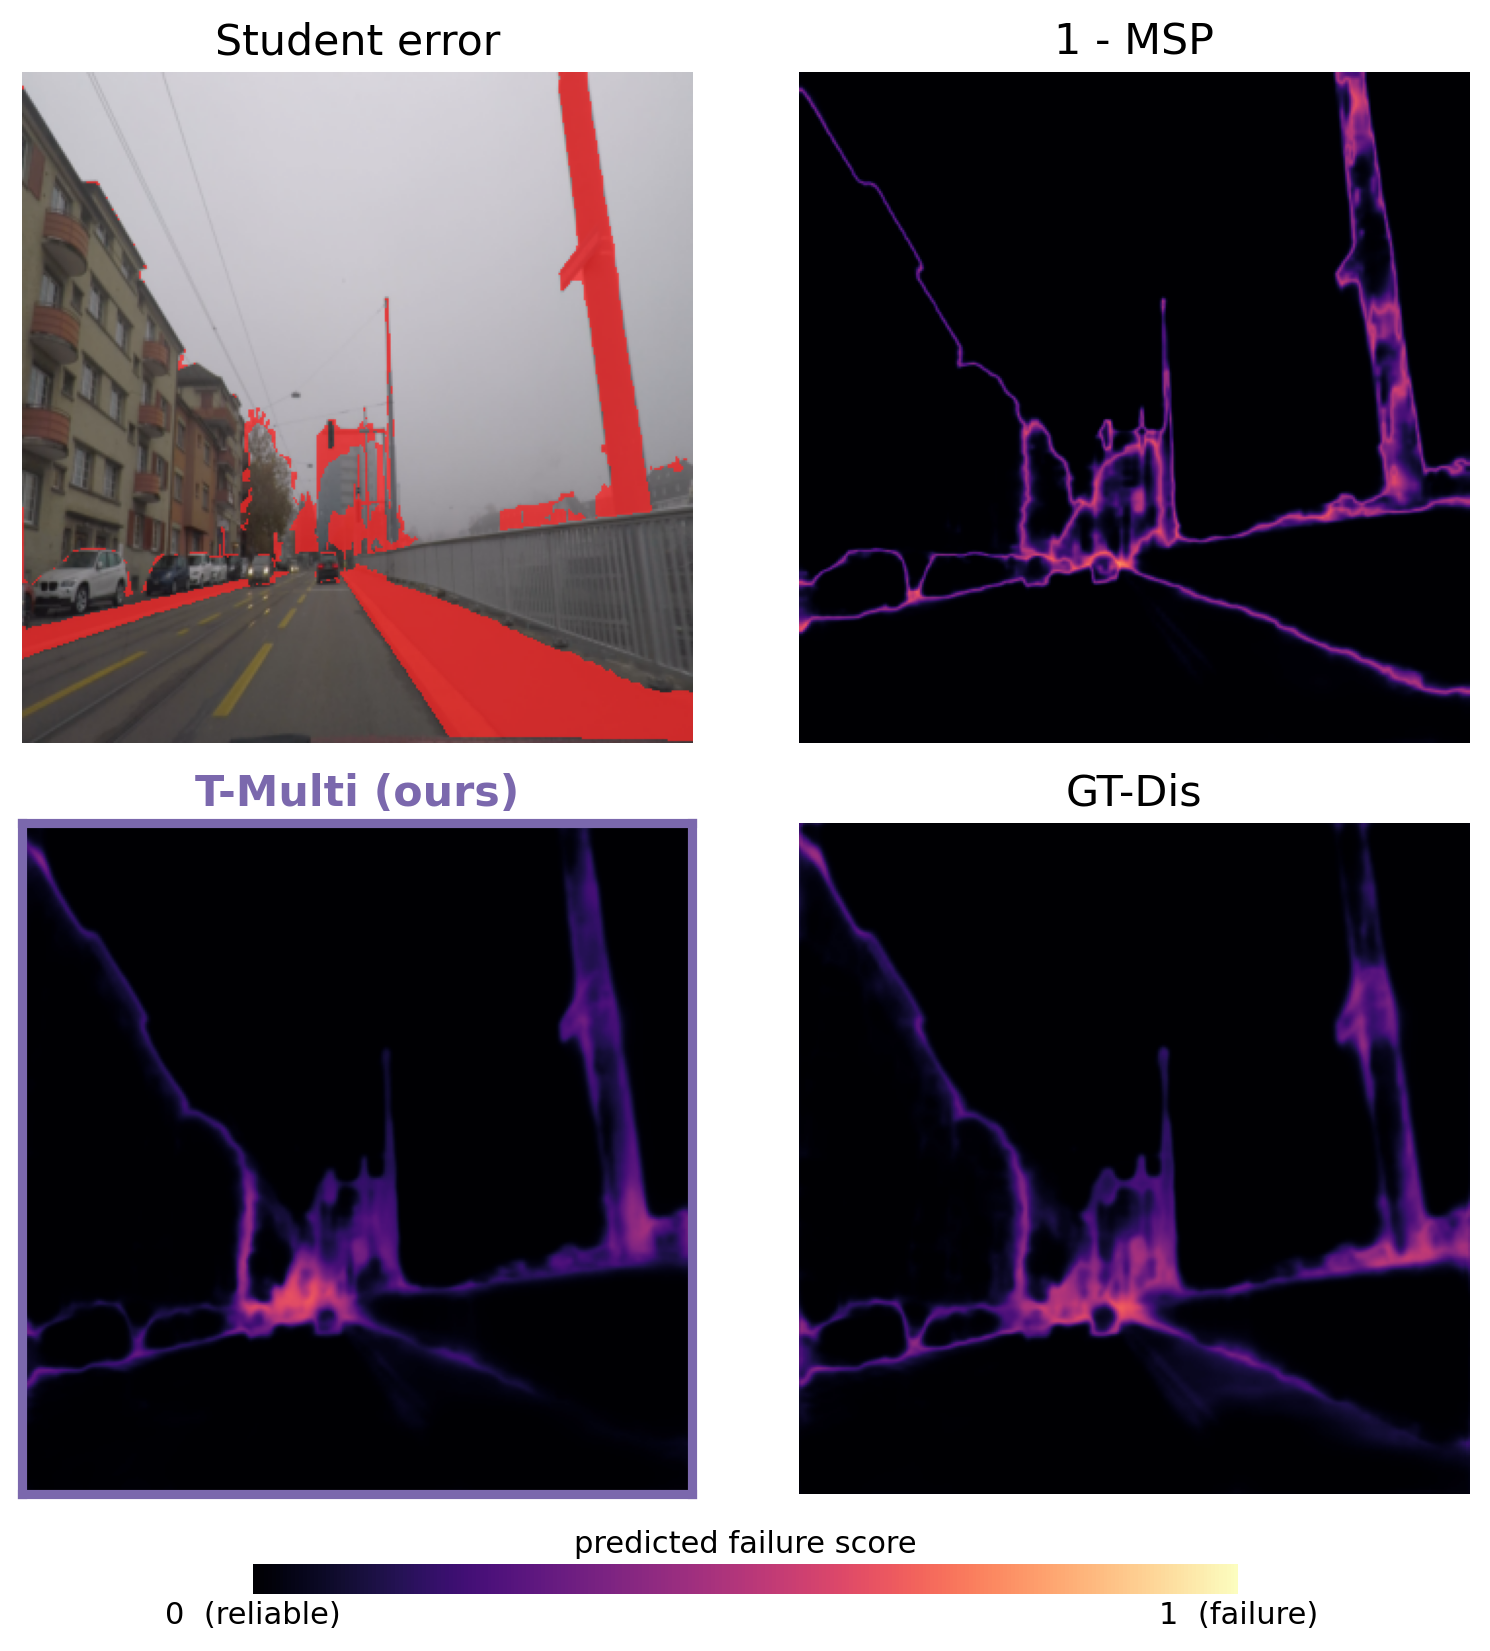
\includegraphics[width=1.0\linewidth]{fig_acdc_fog_strong.png}
\caption{Qualitative failure detection on a single ACDC fog example (mit-b1). The first panel overlays student pixel error in red on the input image; the remaining three show the predicted failure scores for $1{-}\mathrm{MSP}$, T-Multi (ours), and the GT-Dis baseline. $1{-}\mathrm{MSP}$ activates almost exclusively along object boundaries and misses the interior regions where the student fails. Both learned heads recover the boundary structure and additionally fire on failed interiors, where silent confident failures are most spatially concentrated. Colours show each method's relative score within its own panel and are not comparable in absolute terms across panels.}
\label{fig:snow-qual}
\end{figure}


\section{Risk-coverage curves}

\begin{figure}[H]
\centering
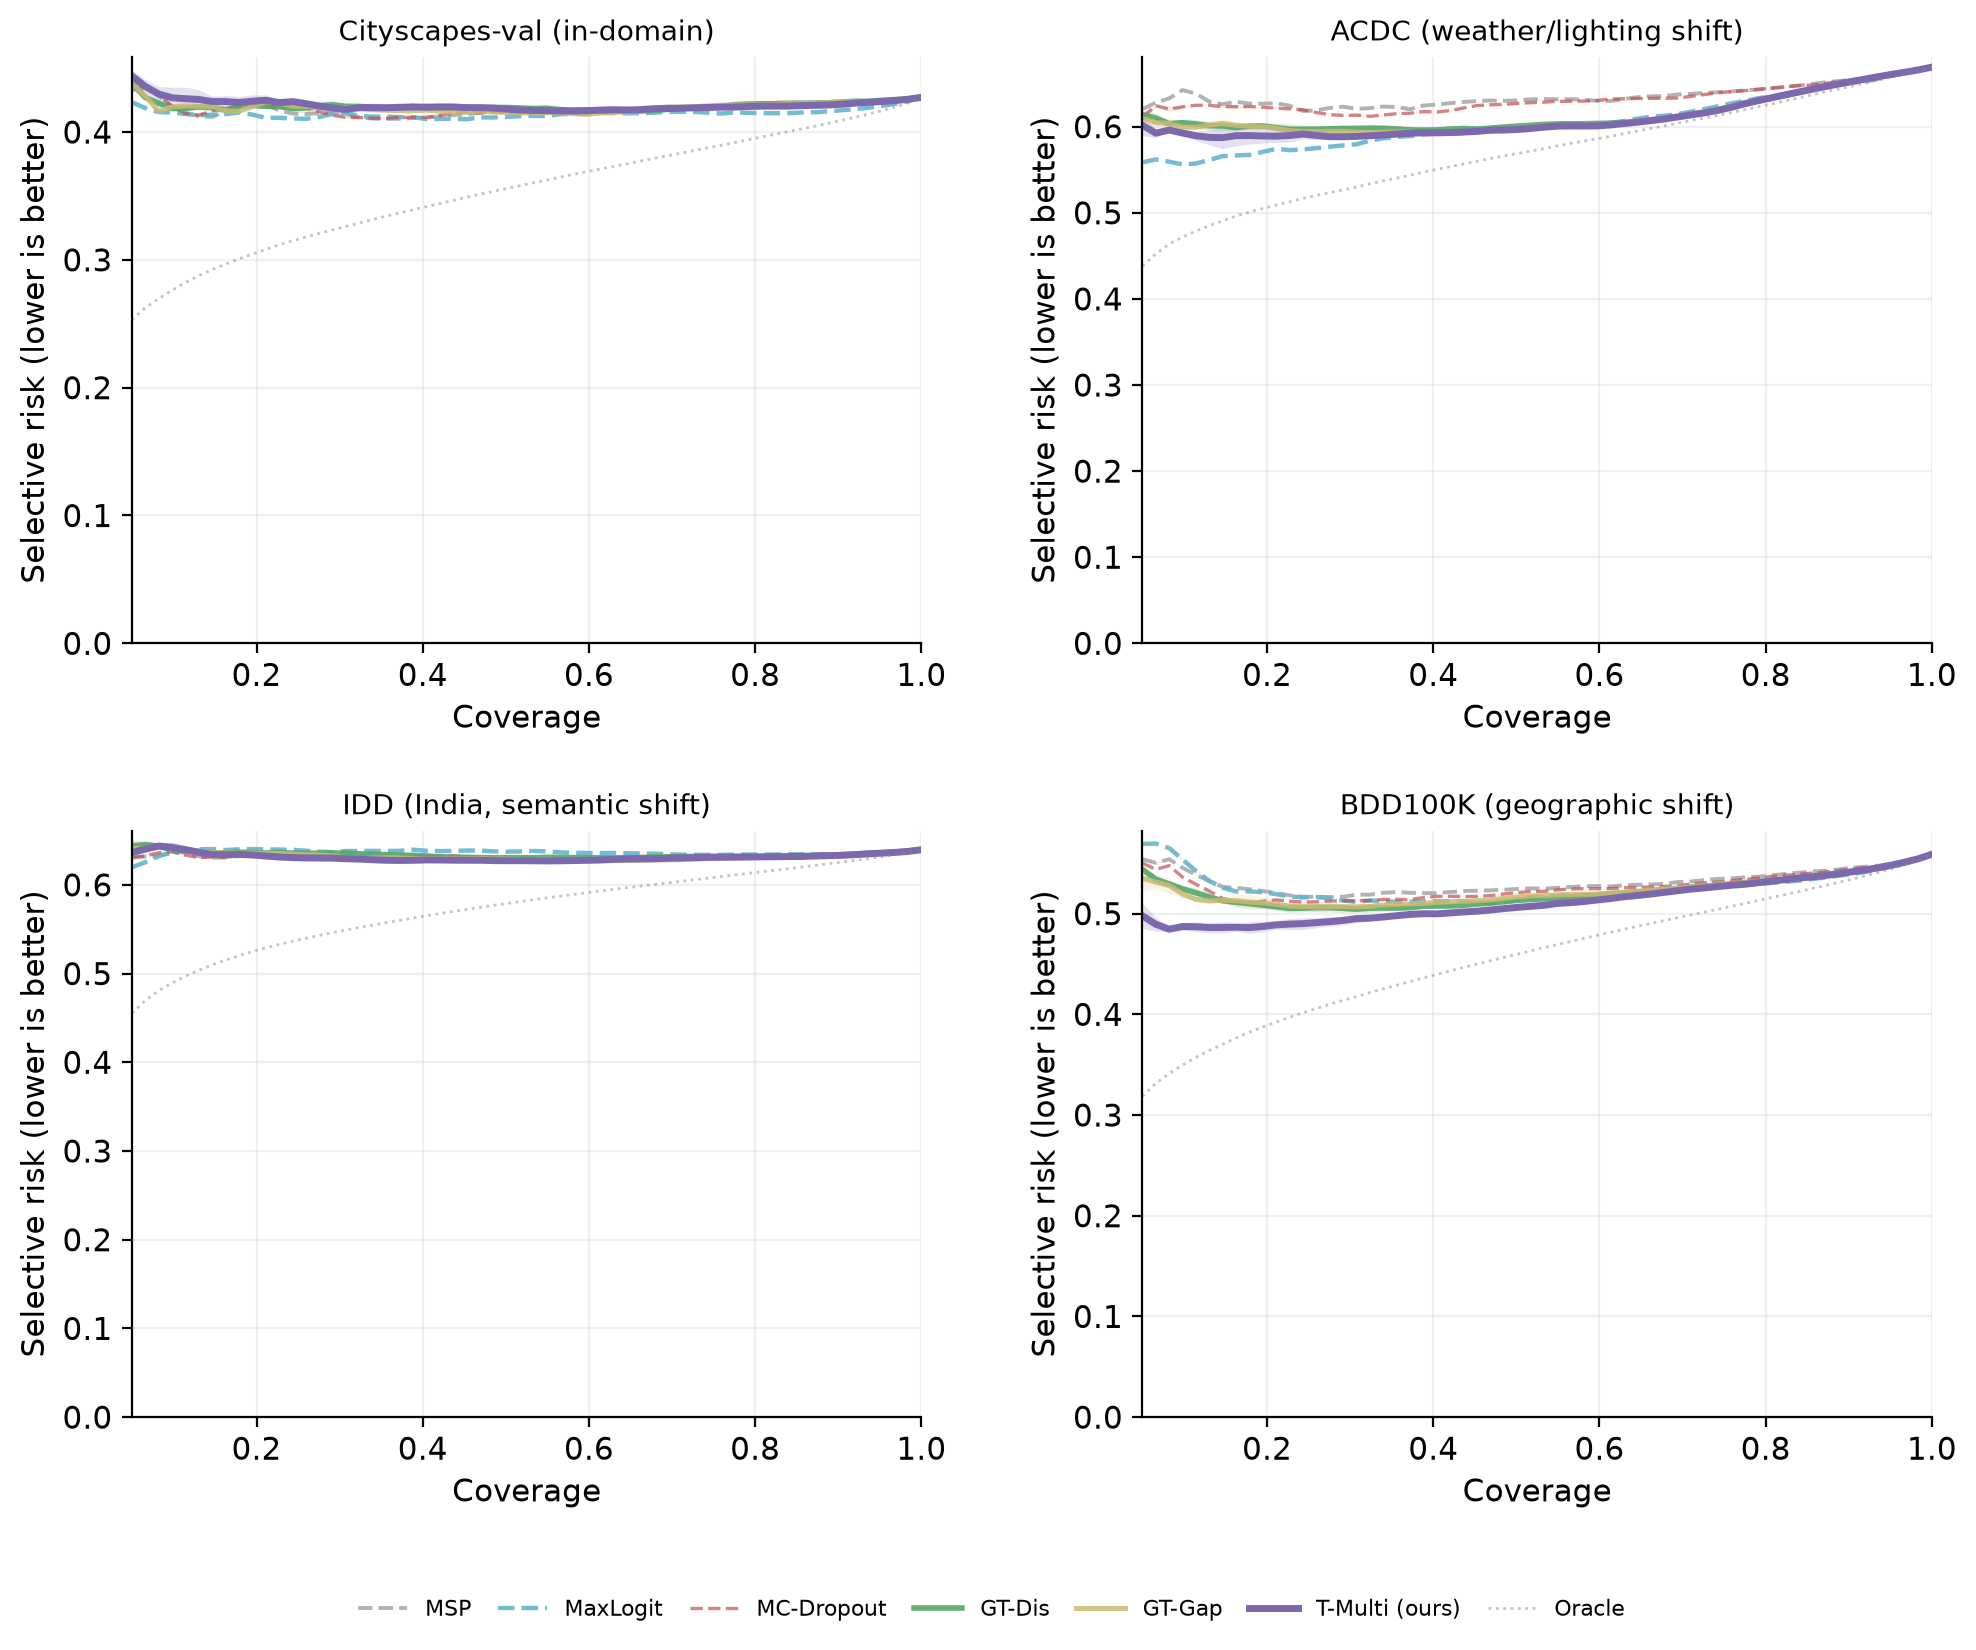
\includegraphics[width=0.9\linewidth]{fig_risk_coverage.png}
\caption{Risk-coverage curves (mit-b1). T-Multi is competitive with GT baselines on ACDC and achieves the lowest selective risk on BDD. The Oracle curve orders images by their true risk ($1-\mathrm{mIoU}$) and lower-bounds the achievable selective risk.}
\label{fig:rc}
\end{figure}


\section{Implementation details}
\label{app:impl}

\paragraph{Guardrail architecture.} For an input of $19$ student logits concatenated with the student's decoder feature map ($F$ channels; $F{=}256$ for b0, $512$ for b1/b2, bilinearly resized to the logit resolution), the head is:
\begin{itemize}
\item \texttt{conv1}: $\mathrm{Conv2d}(19{+}F \to 64, 3{\times}3, \text{pad }1)$, then BatchNorm2d, ReLU;
\item \texttt{conv2}: $\mathrm{Conv2d}(64 \to 64, 3{\times}3, \text{pad }1)$, then BatchNorm2d, ReLU;
\item \texttt{conv3}: $\mathrm{Conv2d}(64 \to 32, 3{\times}3, \text{pad }1)$, then BatchNorm2d, ReLU;
\item two output heads: \texttt{disagree\_head} $=\mathrm{Conv2d}(32 \to 1, 1{\times}1)$ and \texttt{gap\_head} $=\mathrm{Conv2d}(32 \to 1, 1{\times}1)$; a $\mathrm{Linear}(32\to 1)$ scalar head over global-average-pooled features exists but is trained only for the scalar-benefit control.
\end{itemize}
All convolutions use bias and default (Kaiming-uniform) initialization; there is no dropout. Totals: $214{,}275$ parameters for b0 and $361{,}731$ for b1/b2 (the confidence-feature variant adds $2$ input channels, i.e.\ $+1{,}152$). The head is fully convolutional, so $\hat d,\hat s$ are produced at the logit resolution.

\paragraph{Training.} Stage-4 guardrail training freezes the student and teacher. Losses are masked-mean over valid pixels: binary cross-entropy with logits for $\hat d$ and smooth-$\ell_1$ for $\hat s$, with equal weights $\lambda_{\mathrm{dis}}{=}\lambda_{\mathrm{risk}}{=}1.0$; the BCE is unweighted and the severity targets are not clipped or normalized. Optimizer AdamW ($\text{lr}{=}10^{-3}$, weight decay $10^{-3}$), cosine schedule, $50$ epochs, batch size $8$, crop $512{\times}1024$, mixed precision, seed $42$ (plus $137,256$ for multi-seed). Online corruption augmentation is applied per image with probability $0.5$, drawing one family from \{underexposure, motion blur, noise, fog\} at severity $\sim\mathcal{U}[0.2,0.8]$; teacher and student are re-evaluated on the corrupted image so the targets match the input seen by $G$.

\paragraph{Baseline scores.} Every method reduces a dense per-pixel map to an image-level score by averaging over the same valid (non-ignore) pixels; higher score $=$ more likely failure. \textbf{MSP}: risk $=1-$ mean per-pixel max-softmax. \textbf{Entropy}: mean per-pixel softmax entropy. \textbf{MaxLogit}: risk $=-$ mean per-pixel maximum logit. \textbf{Energy}: mean per-pixel $-\log\sum_c\exp z^S_{ijc}$ at temperature $1$. \textbf{Temperature-scaled MSP}: MSP after dividing logits by a \emph{fixed} $T{=}2$ (not tuned on any split). \textbf{MC-Dropout}: predictive entropy of the mean softmax over $4$ stochastic passes. \textbf{Deep Ensemble}: predictive entropy of the mean softmax over $3$ students (the seed-$42$ student plus two independently trained seed-$137/256$ students).

\paragraph{AURC.} With images sorted by descending confidence, the selective risk at coverage $c{=}k/N$ is $R(c)=\tfrac1k\sum_{i\le k} \rho_{(i)}$ where $\rho=1-\mathrm{mIoU}$; $\mathrm{AURC}=\int_0^1 R(c)\,dc$ by the trapezoid rule over the full $N$-point coverage grid (lower is better). This is the conventional AURC, distinct from AUGRC~\citep{traub2024overcoming}.

\paragraph{Datasets and label mappings.} All models are trained on Cityscapes; temperature scaling is not fit on Cityscapes-val or any other split. IDD and BDD labels are mapped to the $19$ Cityscapes classes, and pixels with no corresponding class are set to the ignore index ($255$) and excluded from every metric and score, as are ACDC's ignore regions. BDD100K evaluation uses a fixed $1{,}000$-image validation subset.


\section{Assets and licenses}
\label{app:assets-licenses}
We use existing datasets and pretrained models only under their original terms. Cityscapes is used for training and in-domain evaluation. ACDC is used for adverse-condition evaluation and is used under the official ACDC license for non-commercial use. IDD is used for geographic and semantic shift evaluation and is accessed through the official IDD portal. BDD100K is used for geographic and environmental shift evaluation under the official BDD100K terms. The SegFormer teacher and student architectures are based on the SegFormer model family, and the pretrained NVIDIA Hugging Face checkpoint used is licensed under the terms listed in the model card.

Released code is distributed under the repository license. Released checkpoints are provided for research use and remain subject to upstream model and dataset terms and do not include or redistribute raw dataset images or labels.


\end{document}
